%%%%%
%%%%%  Use LUALATEX, not LATEX.
%%%%%
%%%%
\documentclass[]{VUMIFTemplateClass}

\usepackage{indentfirst}
\usepackage{amsmath, amsthm, amssymb, amsfonts}
\usepackage{mathtools}
\usepackage{physics}
\usepackage{graphicx}
\usepackage{verbatim}
\usepackage[hidelinks]{hyperref}
\usepackage{color,algorithm,algorithmic}

\usepackage{xcolor}
\usepackage{tcolorbox}

\newcommand{\yellowcomment}[1]{%
    \begin{tcolorbox}[colback=yellow!80, colframe=yellow!80, arc=0pt, outer arc=0pt, boxrule=0pt, left=3pt, right=3pt, top=3pt, bottom=3pt]
        \textbf{\textcolor{red}{COMMENT:}} #1
    \end{tcolorbox}
}

% Alternative using colorbox with parbox for inline comments
\newcommand{\inlineyellow}[1]{%
    \colorbox{yellow!80}{\parbox{\dimexpr\textwidth-2\fboxsep}{%
        \textbf{\textcolor{red}{COMMENT:}} #1%
    }}%
}

% Even more obnoxious version with red border
\newcommand{\warningcomment}[1]{%
    \begin{tcolorbox}[colback=yellow!90, colframe=red, arc=0pt, outer arc=0pt, boxrule=2pt, left=5pt, right=5pt, top=5pt, bottom=5pt]
        \Large\textbf{\textcolor{red}{FIX THIS: }} \normalsize #1
    \end{tcolorbox}
}

\newcommand{\goodcomment}[1]{%
    \begin{tcolorbox}[colback=green!20, colframe=green!60, arc=0pt, outer arc=0pt, boxrule=1pt, left=3pt, right=3pt, top=3pt, bottom=3pt]
        \textbf{\textcolor{green!70!black}{GOOD:}} #1
    \end{tcolorbox}
}

\newcommand{\noticecomment}[1]{%
    \begin{tcolorbox}[colback=blue!20, colframe=blue!60, arc=0pt, outer arc=0pt, boxrule=1pt, left=3pt, right=3pt, top=3pt, bottom=3pt]
        \textbf{\textcolor{blue!70!black}{NOTE:}} #1
    \end{tcolorbox}
}

% Inline version for positive comments
\newcommand{\inlinegreen}[1]{%
    \colorbox{green!20}{\textbf{\textcolor{green!70!black}{✓ GOOD:}} #1}%
}

\newcommand{\todocomment}[1]{%
    \begin{tcolorbox}[colback=red!20, colframe=red!60, arc=0pt, outer arc=0pt, boxrule=1pt, left=3pt, right=3pt, top=3pt, bottom=3pt]
        \textbf{\textcolor{orange!70!black}{TODO:}} #1
    \end{tcolorbox}
}

\newcommand{\suggestioncomment}[1]{%
    \definecolor{lime}{RGB}{50,205,50}%
    \begin{tcolorbox}[colback=lime!15, colframe=lime!60, arc=0pt, outer arc=0pt, boxrule=1pt, left=3pt, right=3pt, top=3pt, bottom=3pt]
        \textbf{\textcolor{lime!70!black}{SUGGESTION:}} #1
    \end{tcolorbox}%
}

\usepackage[nottoc]{tocbibind}
\usepackage{tocloft}

\usepackage{amssymb}

\usepackage{titlesec}
\newcommand{\sectionbreak}{\clearpage}

\usepackage{titlesec}

\setcounter{secnumdepth}{4}
\setcounter{tocdepth}{3}

\titleformat{\paragraph}
{\normalfont\normalsize\bfseries}{\theparagraph}{1em}{}
\titlespacing*{\paragraph}
{0pt}{3.25ex plus 1ex minus .2ex}{1.5ex plus .2ex}

% Create the custom command
\newcommand{\subsubsubsection}[1]{\paragraph{#1}}

\makeatletter
\renewcommand{\fnum@algorithm}{\thealgorithm}
\makeatother
\renewcommand\thealgorithm{\arabic{algorithm} algorithm}

\usepackage{biblatex}
\bibliography{bibliografija}
%% to change the numbering (numeric or alphabetic) of bibliographic sources, make the change in VUMIFTemplateClass.cls, line 139

% Author's MACROS
\newcommand{\EE}{\mathbb{E}\,} % Mean
\newcommand{\ee}{{\mathrm e}}  % nice exponent
\newcommand{\RR}{\mathbb{R}}




\studyprogramme{Software engineering} %Write your study 


% pilnas pavadinimas, aiskina ka visa tai daro
% prasmingas pavadinimas cia
\worktitle{\textit{UniServe}: A Universal Service Management Platform for Reservation and Order-Based Businesses} 
\workauthor{Tadas Riksas, Darius Spruogis, Gustas Mickus, Kajus Bicka}

\supervisor{Kristina Lapin}

\begin{document}
\selectlanguage{english}

\onehalfspacing
\begin{titlepage}
\vskip 20pt
\begin{center}

\includegraphics[scale=0.55]{images/MIF.png}
\end{center}

\makeatletter

\vskip 20pt
\centerline{\bf \large \textbf{VILNIUS UNIVERSITY}}
\vskip 10pt
\centerline{\large \textbf{FACULTY OF MATHEMATICS AND INFORMATICS}}
\vskip 10pt
\centerline{\large \textbf{\MakeUppercase{\@studyprogramme \space study programme}}}

\vskip 80pt
\centerline{\Large \@worktype}
\vskip 20pt
\begin{center}
    {\bf \LARGE \@worktitle}
\end{center}
\begin{center}
    {\bf \Large \@secondworktitle}
\end{center}
\vskip 80pt

\centering{\Large \@workauthor}
\@ifundefined{@secondauthor}{}
{
\vskip 10pt
\centering{\Large \@secondauthor}
}
\vskip 20pt

\centering{
    \begin{tabular}{rcp{.7\textwidth}}
        {\Large Supervisor} & {\Large :} & {\Large \@supervisor}\\[10pt]
        \@ifundefined{@scientificadvisor}{}
            {
                {\Large Scientific advisor} & {\Large :} & {\Large \@scientificadvisor}\\[10pt]
            }
        \@ifundefined{@reviewer}{}
            {
                {\Large Reviewer} & {\Large :} & {\Large \@reviewer}\\[10pt]
            }
    \end{tabular}}


\vskip 110pt

\centerline{\large \textbf{Vilnius}}
\centerline{\large \textbf{\the\year{}}}

\makeatother

\newpage
\end{titlepage}
%\newgeometry{top=2cm,bottom=2cm,right=2cm,left=3cm}
\setcounter{page}{2}


\singlespacing
\selectlanguage{english}
% list of figures, delete if not needed
% \listoffigures 

%list of tables, delete if not needed
% \listoftables

\tableofcontents
\onehalfspacing


% \section*{Check List \checkmark}

% \section*{Assignment Requirements}

% \subsection*{Documentation Requirements}

% The assignment consists of the following parts: title page, table of contents,
% and the main part.

% \textbf{Section numbering.} Headings of the sections must be numbered strictly
% hierarchically. The sections have assigned numbers, such as 1., subsections –
% 1.1., 1.2, subsubsections – 1.1.1., 1.1.2. and so on. \checkmark

% \textbf{File naming requirements.} A file name contains a short project title,
% an assignment number and an assignment title. Example: CarBuddy 1 User needs.pdf

% \subsection*{An outline of the main part}

% \begin{enumerate}
%     \item Introduction \checkmark
%     \begin{enumerate}
%         \item[1.1.] Project titles \checkmark
%         \item[1.2.] Problem statement \checkmark
%     \end{enumerate}
    
%     \item User needs analysis
%     \begin{enumerate}
%         \item[2.1.] Expectations of the stakeholders \checkmark
%         \item[2.2.] $\langle$The name of the first user group$\rangle$ research \{for each user group in both primary and secondary stakeholders\} \checkmark
%         \begin{enumerate}
%             \item[2.2.1.] Current users' activities \checkmark
%             \begin{enumerate}
%                 \item[2.2.1.1.] $\langle$Title of the 1st user story$\rangle$ \checkmark
%                 \begin{itemize}
%                     \item Description of current activity (unnumbered subsection) \checkmark
%                     \item Problems and opportunities (unnumbered subsection) \checkmark
%                 \end{itemize}
%                 \item[2.2.1.2.] $\langle$Title of the 2nd user story$\rangle$ \checkmark
%                 \begin{itemize}
%                     \item \ldots \checkmark
%                 \end{itemize}
%             \end{enumerate}
%             \item[2.2.2.] Characteristics of the people, activities, context, and technologies \checkmark
%             \item[2.2.3.] Needs
%             \item[2.2.4.] Usability objectives
%         \end{enumerate}
%         \item[2.3.] $\langle$The name of the next user group$\rangle$ needs analysis \{if needed\}
%         \item[] \ldots
%         \item[2.$\langle$n+1$\rangle$.] Inspiring user interface designs
%     \end{enumerate}
% \end{enumerate}

% \subsection*{Explanations}

% \textbf{The title page} contains:
% \begin{itemize}
%     \item university name, faculty, and study program, \checkmark
%     \item project full title, \checkmark
%     \item contributors' names and surnames, \checkmark
%     \item year. \checkmark
% \end{itemize}

% \textbf{The table of contents} includes the sections and subsections until the 3rd level and page numbers. \checkmark

% \textbf{Project titles.} The project must have two titles: \checkmark
% \begin{itemize} 
%     \item full (e.g. ``Vilnius University Library App'') and \checkmark
%     \item short (e.g. ``Library''). \checkmark
% \end{itemize}

% The full title is used on the title page and in this section, a short title serves as a project reference in the document text and assignment file names. \checkmark

% \textbf{Problem statement} explains the high-level project goals shortly and
% specifically (about half a page). The problem is described in terms of user
% activities and situations where the problem occurs, and what aspects might be
% improved with a technical solution. Avoid describing or suggesting a solution at
% this stage that will hamper your design thinking when you start solving the
% problem. \checkmark

% To gather the relevant facts for your problem statement, you can use a simple
% technique called the 6 Ws, which involves answering the questions below: \checkmark
% \begin{itemize}
%     \item Who is affected by the problem? \checkmark
%     \item What is the problem? \checkmark
%     \item Where does this problem occur? \checkmark
%     \item When does the problem occur? \checkmark
%     \item Why does the problem occur? \checkmark
%     \item Why is the problem important? \checkmark
% \end{itemize}

% \textbf{Expectations of the stakeholders} \checkmark

% Specify the specific groups of people (stakeholders) involved in activities that
% will be supported by your project (see Lecture 1. User-centered design).
% Identify relevant stakeholders' intentions that are supposed to be fulfilled. In
% the competitors subsection, you should list your closest competitors. Then you
% should list your main competitive advantages over them. \checkmark

% \textbf{Current user activities} \checkmark

% Watching how people do things is a great way to learn their goals and values,
% and come up with design insight. This is called user research. This assignment
% helps you train your eyes and ears to develop design ideas. Your goal is to
% uncover user needs, breakdowns, clever hacks, and opportunities for improvement.
% Begin by selecting a specific activity to observe. \checkmark

% The description contains the user story that tells about the current user
% activities. Note that your service or product does not exist yet. Therefore, you
% must describe the existing activities, such as how your users achieve their
% goals with existing competitive products, and highlight the pain points and
% troubles. Then, indicate the problems and improvement opportunities (see the
% assignment outline). \checkmark

% Describe at least 3 observations of current user activities for primary users,
% for the secondary – there can be fewer. Examples of activity descriptions: \checkmark

% \begin{itemize}
%     \item \textbf{Story 1:} Ann is a clerk in her twenties, comes for a quick
%     lunch. She wants to see dishes that are served within 15 min. She waits 10
%     min. for a waiter. The waiter says that only soup can be served in 15 min.
%     Therefore Ann leaves the restaurant and goes for a fast food nearby. \checkmark
    
%     \item \textbf{Story 2:} Andrew, a thirty-two-year-old restaurant client, who
%     suffers from allergies, comes to a restaurant. He examines the menu. The
%     menu is long, ingredients are mentioned in every dish. So, it takes about 5
%     minutes to choose a dish. Waiting for the dish takes 20 min. Andrew must
%     hurry and eats quickly because he has to return to work on time. \checkmark
    
%     \item \textbf{Story 3:} Thirty-five-years-old Peter goes to a restaurant
%     with his family. He noticed on Google Maps that a new restaurant was opening
%     not far away. They spend time reading the menu. The café has a children's
%     menu, but children's favorite dishes are missing. Children are bored because
%     of missing the game area. The family chooses quick dishes from the menu. \checkmark
    
%     \item \textbf{Story 4:} Fourty-year-old Sara comes with her friends to a
%     restaurant on Sunday. They are looking for a big table but see that the
%     restaurant is almost full. They started to explore the TripAdvisor app on
%     their phone for other restaurants phone numbers to ask whether they have a
%     free big table for a group. \ldots \checkmark
% \end{itemize}

% \textbf{How to check whether a story is correct?} \checkmark

% A story should cover
% characteristics of peoples, activities, environment and technologies that are
% related to computerized activities. If any characteristic is missing, you should
% augment the story. \checkmark

% \textbf{Needs statements and usability objectives} 
 
% After describing user stories, go over your findings. Brainstorm about both user
% needs and usability objectives. Observe the opportunities for design innovation
% that would improve the activity. User needs are formulated for primary and
% secondary users, only. Indirect stakeholders formulate business goals that are
% abstract and relate to business strategy. Business goals should be met with the
% needs of primary and secondary users. The impact of business goals on user needs
% is explained in Lecture 2, slides 52–53. Examples of usability goals and needs
% are provided in slides 54--57, and usability objectives are tackled in slides
% 58--60. 

% The project must contain at least 15 user needs. 3–5 usability objectives are
% defined for every user group. You are not looking for solutions yet: focus on
% user needs only. User needs and usability objectives must have unique
% identifiers. Below the needs and the usability objectives provide traceability
% matrices that link the need or objective identifier with the number of paragraph
% of the user story from which it is derived.

% \textbf{Inspiring user interface designs}

% Provide here examples of successful user interface solutions of existing
% software that can be useful for specified user needs and usability objectives.
% Provide a screenshot of the design, the number of user needs, or the usability
% objective for which this solution would be beneficial. Images should have
% captions with concise explanations and references to the source, from which this
% image is taken. The text related to the image should contain cross-reference to
% the image. Provide at least 5 examples.

% \section*{Other}

% \subsubsection*{Use of AI}

% Just a little note: dont just copy the assignment text and expect good output,
% look into slides also and try to apply lecture material. 

% \subsubsection*{Comments}

% \warningcomment{This is a very important comment}
% \yellowcomment{This is a comment}
% \todocomment{This is a todo comment}
% \noticecomment{This is a notice comment}
% \goodcomment{This is a good comment}
% \suggestioncomment{This is a suggestion comment}

% Usage of comments in text is recommended as it helps to highlight problems and
% solutions. The Overleaf comments are often ignored, therefore, it is recommended
% to use the comments defined in this template.

\section{Introduction}
\subsection{Project title}

\textbf{Full title:} \textit{UniServe: A Universal Service Management Platform for Reservation and Order-Based Businesses}

\textbf{Short title:} \textit{UniServe}


\textbf{Explanation:} "Uni" represents \emph{universal}, indicating the platform's flexibility across a variety of business models 
(reservation based businesses such as massage services or order based businesses such as restaurants). 
"Serve" refers to \emph{service}, emphasizing the platform’s role in providing core functionalities for these types of businesses.

\subsection{Problem statement}

Traditional methods of managing reservations and orders—such as handwritten
appointment books, paper-based inventory tracking, manual payment processing,
and physical order documentation—create significant operational bottlenecks that
directly impact business performance and stakeholder satisfaction. Reliance on
outdated manual processes for tracking orders, services, inventory, payments,
and taxes create several critical problems:

\begin{itemize}
    \item \textbf{For employees:} Manual order-taking and appointment booking
    requires constant \textbf{memorization} of availability, pricing, and menu
    details. Staff must physically check excel/paper schedules or call to verify
    bookings, leading to \textbf{errors}, double-bookings, and frustrated
    customers. During peak periods (weekends, holidays, promotional events),
    employees become \textbf{overwhelmed} managing multiple phone lines while
    \textbf{simultaneously serving} in-person customers, \textbf{calculating
    totals}, \textbf{managing inventory}, resulting in poor service quality and
    increased stress.

    \item \textbf{For customers:} Manual excel/paper-based systems create
    \textbf{longer wait times} as employees must physically write orders, search
    through paper schedules, and handle multiple forms or cards during each
    transaction. Customers experience \textbf{increased likelihood} of lost or
    incorrect orders due to handwriting errors, misplaced papers, or
    miscommunication between staff members. The \textbf{slower service} caused
    by employees manually searching orders, calculating totals, processing
    appointments leads to customer \textbf{frustration} and
    \textbf{dissatisfaction}, especially during busy periods when paper-based
    workflows create bottlenecks.
    % \todocomment{ask PS design lecturer if users should be able to view that information or if the interface remains the same and simply the employees have access to that information}

    \item \textbf{For business owners:} Manual systems prevent access to crucial
    business data—owners \textbf{cannot easily} track popular items, peak hours,
    or customer patterns. Inventory management and supply chain logistics relies
    on \textbf{guesswork}, leading to waste or stockouts. \textbf{Tax
    management} becomes complicated and error-prone when relying on scattered
    paper receipts and handwritten records. Without automated processes,
    businesses require more staff hours for administrative tasks that could be
    automated, increasing labor costs while \textbf{limiting growth potential}.
\end{itemize}

\textbf{Technical barriers:}

Limited budgets and lack of technical expertise prevent these businesses from
developing in-house solutions as these solutions are often expensive and complex.

\textbf{Why this problem matters and consequences of inaction:}

These manual processes directly limit how much revenue a business can generate.
When employees spend time on paperwork instead of serving customers, the
business serves fewer people and makes less money. The problem gets worse
during busy periods when potential customers leave due to long wait times,
representing direct lost sales. Over time, businesses using manual systems
fall further behind competitors who adopted digital tools—they cannot match
their speed, cannot reduce their costs, and cannot grow at the same rate.
Without change, the gap widens: competitors continue improving their
efficiency while manual-dependent businesses remain stuck with the same
limitations, eventually losing market share and facing reduced profitability
that threatens long-term viability.


\section{Stakeholder analysis}

\subsection{Identifying stakeholders}

\begin{table}[h]
  \centering
  \caption{Stakeholders identification}
  \begin{tabular}{|c|c|}
    \hline
    Stakeholder type    & Stakeholders \\ \hline
    Primary             & Employees, customers \\ \hline
    Secondary           & Client business owners \\ \hline
    Indirect (tertiary) & App business owners \\ \hline
    External/competitors & Square, Toast POS, Restaurant365 \\ \hline
    Technical support   & Sysadmins, tech support \\ \hline
  \end{tabular}
  \label{tab:stakeholders}
\end{table}

% Nielsen‘s principles
% 1. Learnability
% 2. Efficiency of use
% 3. Memorability
% 4. Few and non-
% catastrophic errors
% 5. Satisfaction

\textbf{Primary stakeholders:}
\begin{itemize}
    \item \textbf{Employees} expect a system that eliminates the need to
    memorize constantly changing information (availability, pricing, specials),
    allows calculating totals and managing inventory efficiently, reduces the
    risk of errors in bookings and order processing, and allows for a more
    satisfying and efficient customer serving experience.
    % \item \textcolor{gray}{\textbf{Employees} expect a system that removes the
    % need to memorize, provides quick access to changing information (item
    % availability, pricing, specials), automates calculations (discounts, split
    % bills, etc.), validates orders and bookings.}
    
    % \warningcomment{from lecture: "So, you don't need to think of self-service,
    % maybe like Burger King or McDonald's", "...you can assume that all business
    % operations are performed by business employees. So, you don't need to worry
    % that much about customer accounts..."}

\end{itemize}

\textbf{Secondary stakeholders:}
\begin{itemize}
    % o sitie primary? jie interactina su musu sistemos UI???? Jie interactina, bet pagal primary users apibrezima jie turetu intereactinti frequently, o owners ocasionally - tai secondary turetu buti manau
    \item \textbf{Client business owners} expect automated access to business
    data (sales patterns, inventory levels, customer analytics, tax information)
    that are error-free, reduced administrative overhead. They expect efficient
    systems that will reduce labor and allow them to focus on strategic
    decision-making and preserving historical records—to help identify trends,
    and boost overall profits.
    % not sure ar cia geriau, bet bandau kazkaip labiau specific kelis ir pateikti examples
    % \item \textcolor{gray}{\textbf{Client business owners} expect a system that
    % accelerates employee-managed orders and reservations, for example through
    % automatic validation or menu management (e.g., limiting options when items
    % are out of stock). They also expect actionable data—such as tracking sales,
    % payments, discounts, tips, and preserving historical records—to help
    % identify trends, improve inventory management, and boost overall profits.}
    
    \item \textbf{Customers} expect satisfying and efficient service with minimal wait times during ordering and booking. They expect their orders and appointments to be accurately recorded, with clear confirmations for bookings and orders. They expect to see available menu items in real time to make choices quickly.

    % \item \textcolor{gray}{\textbf{Customers} expect quick ordering and booking
    % with accurate records, and no inconveniences like being told later that an
    % item is unavailable or an appointment was entered incorrectly.}

\end{itemize}

\textbf{Indirect (tertiary) stakeholders:}
\begin{itemize}
    \item \textbf{App business owners} recognize a market opportunity to serve
    underserved small and medium businesses that cannot afford or implement
    complex enterprise solutions. They want steady income growth by capturing
    market share from businesses currently using manual processes or considering
    expensive alternatives.
    % \item \textcolor{gray}{\textbf{App business owners} expect to capture market
    % share from small and medium businesses using manual tools (e.g., Excel) or
    % unable to use more advanced and expensive solutions (e.g., Toast POS). They
    % expect steady income growth by attracting these customers.}


\end{itemize}


\textbf{Competitors:}

\begin{itemize}
    \item Square
\begin{itemize}
        \item \textbf{COMPETITOR ANALYSIS:}
        
        Square offers a free basic POS system with no monthly fees, appealing to
        small businesses starting out. However, Square charges per-transaction
        fees that accumulate for high-volume businesses. Users report that the Square SMS reminders for appointments feature is incomplete and unavailable for some plans.

        \item \textbf{OUR ADVANTAGES:} 
        
        Our flat-rate pricing model provides cost predictability for growing
        businesses without per-transaction fees. We offer SMS reminders for customer appointments for all plans.

    \end{itemize}
    

    \item {Toast POS}
    \begin{itemize}
        \item  \textbf{COMPETITOR ANALYSIS:}
        Toast is a restaurant-specific system with strong
        features for food service operations. However, Toast requires significant
        upfront investment in proprietary hardware (costing \$494-\$1,034) and monthly
        software fees starting at \$69 for advanced features. This pricing model
        puts it out of reach for many small restaurants operating on tight margins.
        Toast also requires technical staff to setup.

        \item  \textbf{OUR ADVANTAGES:} 
        We offer lower upfront costs by working with
        standard devices businesses may already own. Our simplified interface
        requires minimal training, allowing staff to start using the system
        immediately without dedicated technical support or lengthy onboarding
        processes.
    \end{itemize}
    
    \item Restaurant365
    \begin{itemize}
        \item \textbf{COMPETITOR ANALYSIS:}
        Restaurant365 provides comprehensive
        accounting and operations management with deep financial reporting
        capabilities. However, it starts at $90-$249 per location per month, making
        it expensive for single-location small businesses. The system is built for
        restaurant groups managing multiple locations and complex accounting needs,
        offering far more features than small businesses require. This complexity
        makes it difficult to learn and overkill for businesses that simply need
        basic order management and inventory tracking.

        \item \textbf{OUR ADVANTAGES:} 
        We focus on core operational needs—order taking,
        reservations, basic inventory—without expensive accounting modules that
        small businesses do not need. Our pricing is accessible for single-location
        businesses, and our simplified feature set means owners can understand and
        use the system without accounting expertise.
    \end{itemize}
    

    \item Excel: 
    
    \begin{itemize}
        \item \textbf{COMPETITOR ANALYSIS:}
        Many small businesses currently use Excel spreadsheets
        to manually track orders, inventory, and schedules. Excel is familiar and
        inexpensive, which explains its continued use. However, Excel requires
        businesses to build their own systems from scratch, offers no automation for
        repetitive tasks, and provides no real-time updates when multiple staff
        members need access. Data entry errors are common because everything must be
        typed manually, and there is no way to connect Excel directly to payment
        processing or customer-facing ordering systems.
        
        \item \textbf{OUR ADVANTAGES:} 
        We provide a ready-to-use system with built-in
        templates for common business operations, eliminating the need to build
        tracking systems from scratch. Our system automates repetitive tasks like
        inventory calculations and sales reporting, reduces data entry errors
        through dropdown menus and automated calculations, and allows multiple staff
        members to access updated information in real-time. Our systems are also reliable and do not run on a single
        computer that can crash or be misplaced.
        \end{itemize}
        
\end{itemize}

\textbf{Development and maintenance team:}
\begin{itemize}
    \item \textbf{Sysadmins} expect reliable system architecture that can handle
    varying loads (especially during peak business periods), scalable
    infrastructure to accommodate business growth, and clear deployment
    procedures to maintain system stability.
    \item \textbf{Tech support} expect comprehensive documentation and effective
    troubleshooting tools to efficiently resolve the types of issues small
    business users commonly encounter, along with manageable processes for user
    support that don't overwhelm limited support resources.
\end{itemize}


% <The name of the first user group> research {for each user group in both primary and secondary stakeholders}

% should include people characters, activities, enviroment and technologies or
% in other words it should give info to PACT analysis.          
% Character - who are the users, what are their physical and cognitive abilities,
% Activities - what tasks do they perform, what are their goals, describe the characteristics of tasks
% Context - where and when do they perform these tasks, what are the physical, social, cultural, organizational aspects of the environment
% Technologies - what tools, devices, software do they use to perform their tasks.


\subsection{Employee research}
% some teams have 5 stories, maybe we need more?
% \noticecomment{Mention current competitors in the stories (not all stories, just some)}

\subsubsection{Current users' activities}

\subsubsubsection{Café Barista Managing Orders}
\label{subsubsubsec:barista-orders}

Marius, 21, works as a barista in a busy café. He takes orders at the counter
and writes them on sticky notes for the kitchen. During the morning rush, notes
sometimes fall to the floor or get smudged by spilled drinks. This leads to
wrong orders being prepared, which frustrates customers and wastes ingredients.
Marius tries to keep the counter tidy, but the lack of a structured system makes
mistakes inevitable and thus Marius spends extra time apologizing and remaking
orders, which slows down the queue.

% \yellowcomment{identify problems and opportunities, identify the problem in the story, go immediately to the essence of the problem}

\textbf{PROBLEMS:}

\begin{itemize}
    \item Lost orders due to sticky notes falling or getting smudged
    \item Time and inventory assets wasted on remaking incorrect orders
\end{itemize}

\textbf{OPPORTUNITIES:}

\begin{itemize}
    \item Implement a digital order management system to reduce reliance on sticky notes and minimize lost orders
\end{itemize}


\subsubsubsection{Salon Receptionist Controlling Bookings}
\label{subsubsubsec:salon-receptionist}

Lucille, a receptionist in her twenties, manages a constant stream of appointment calls at a busy beauty salon. She first records bookings by hand in a diary, then re‑enters them into a spreadsheet. On busy days, mistakes often occur, resulting in an average of 1 error per 6 bookings, such as double bookings. Rescheduling requires searching through the diary, which is time‑consuming and makes customers wait. 
\textbf{PROBLEMS:}

\begin{itemize}
    \item High risk of double bookings or missed appointments due to manual entry errors.
    \item Time wasted searching for original bookings in the paper diary.
\end{itemize}

\textbf{OPPORTUNITIES:}
\begin{itemize}
    \item Implement a digital booking system to reduce manual entry errors and
    makes searching for bookings efficient.
\end{itemize}
% \todocomment{if we say that ppl write in excel we need to specify that as a competitor}


\subsubsubsection{Restaurant Manager Handling Discounts}
\label{subsubsubsec:restaurant-discounts}

Youmna, in her early twenties, manages a busy Lebanese restaurant. During weekday promotions, she manually checks eligible dishes (takes around 2–3 minutes per order) and calculates totals for each order (1–2 minutes), slowing service and sometimes causing errors or missed entries.

\textbf{PROBLEMS:}

\begin{itemize}
    \item High risk of incorrect discounts being applied due to manual calculations.
    \item Time wasted searching for eligible dishes on printed lists.
\end{itemize}

\textbf{OPPORTUNITIES:}
\begin{itemize}
    \item Implement a system that automatically calculates totals and display, reducing errors and speeding up service.
    \item Provide quick access to eligible dishes for promotions, eliminating the need to search through printed lists.
\end{itemize}




\subsubsubsection{Bakery Tracking Inventory}
\label{subsubsubsec:bakery-inventory}

Thomas, 26, manages inventory at a small artisan bakery that recently adopted Restaurant365. The system requires multiple steps to log ingredient usage and current stock, making even simple tasks time-consuming and frustrating. Thomas doesn’t need all the advanced features, he simply needs to know when stock is low so he can reorder supplies efficiently.

\textbf{PROBLEMS:}
\begin{itemize}
    \item Complex interface designed for enterprise needs creates confusion for simple daily tasks.
    \item Time wasted navigating unnecessary financial modules to complete basic inventory functions.
\end{itemize}

\textbf{OPPORTUNITIES:}
\begin{itemize}
    \item System updates inventory based on orders, allowing employees to see current stock levels and know when to reorder.
\end{itemize}


\subsubsection{PACT analysis of employees}
    \textbf{People:} Employees are mostly young to mid-career workers (baristas, receptionists, restaurant managers). They multitask under pressure, balancing customer interaction with operational tasks. Some are comfortable with smartphones and PCs. while other rely heavily on paper-based systems, showing varied levels of technical familiarity. They are motivated by efficiency: fewer errors and faster service lead to smoother operations and higher customer satisfaction. There are three types of employees: frontline employees (baristas, receptionists) who are constantly interacting with customers can often get frustrated dealing with plenty of paper orders that get lost or destroyed. Supervisors/managers oversee staff, they need better technology to make calculated decisions regarding discounts, handle exceptions etc. Support staff (kitchen staff, stylists) depend on accurate and timely information passed from the frontline, errors directly affect they output.
    

    \textbf{Activities:} Employees regularly take and manage orders or book and
    reschedule appointments throughout their shifts. They communicate with customers
    about availability, prices, and service options, often handling multiple
    requests simultaneously. These activities happen frequently with short
    durations, creating constant time pressure especially during peak hours. Tasks
    involve multiple steps (greeting, taking order, confirming, processing) where
    employees can pause between customers but must complete each transaction.
    Employees work both individually (appointment servicing) and coordinate with team members (kitchen staff), passing
    information verbally or through notes. The activities are moderately complex as
    they require checking availability, applying discounts, and handling exceptions,
    with errors being critical since they directly impact customer satisfaction and
    operations.
    
    \textbf{Context:} Employees work in a fast-paced, noisy and time-sensitive
environments, where they have constant interactions with both in-person and remote customers. Employees work in crowded spaces where handwritten notes can be smudged or lost. Constant phone calls and reliance on diaries make rescheduling time-consuming. Errors cascade into customer dissatisfaction, which consumes extra time and increase stress for staff.
    
    \textbf{Technologies:} Currently, employees rely mostly on paper-based systems (sticky notes, diaries, printed lists). While Point of Sale (POS) systems do exist, they are often underutilized or lack proper integration with bookings and promotions. In some businesses, Excel or spreadsheets act as makeshift digital tools, but these still require manual updates and duplicate data entry. In cafes, POS systems often only handle billing and do not integrate order-tracking, leading baristas to still use sticky notes. POS competitors may support discount application, but discounts must often be entered manually by staff, creating delays and errors. In other service-based fields, some competitors provide basic booking systems, but many lack real-time rescheduling features. 



\subsubsection{Needs of employees}
\begin{itemize}
    % \item[UN-01] An employee needs a way to record customer orders digitally to avoid damaging them in the fast-paced restaurant environment.
    \item[UN-01]\label{UN-01} An employee needs to record customer orders to avoid damaging them in the fastpaced restaurant.
    % \todocomment{Pati sistema sprendzia tai kad nebutu uzsiklojimu.}
   
    % \item[UN-02] An employee needs a system to manage appointment bookings to avoid double bookings and missed clients while handling incoming calls and customer requests.
    \item[UN-02]\label{UN-02} An employee needs to view available booking slots.

    % \todocomment{vartotojas turi pasakyti kad nuo pirmadienio bus akcija, jis iveda akcijas, kad automatiskai skaiciuos tai aisku. kaip naudos sistema vartotojas, pritaikys ives nuolaidas}
    \item[UN-03]\label{UN-03} An employee needs to enter discounts so that the discounts are correctly applied to the relevant items.

    % \item[UN-03] An employee enters discounts to reduce pricing errors and speed up checkout during peak hours.
    
    \item[UN-04]\label{UN-04} An employee needs to search bookings by customer name to resolve customer queries during ongoing service.
    \item[UN-05]\label{UN-05} An employee needs to see a text message indicating what errors occurred if a recorded order is incorrect so that the errors can be corrected immediately.
    \item[UN-06]\label{UN-06} An employee needs to see the final total for each order, so that they do not have to calculate it manually, reducing errors and saving time.
    % \item[UN-05] An employee needs a system that validates employee input and provides instant feedback to reduce errors and increase speed while servicing customers.
    \item[UN-07]\label{UN-07} An employee needs to see current inventory levels automatically updated based on orders so that they can identify low-stock items and reorder supplies.

\end{itemize}

%because constantly memorizing and manually updating details leads to errors, slower service, and lower customer satisfaction.
\subsubsection{Usability objectives for employees}
% \noticecomment{sita daikta naudosime testavimo metu, ziuresime ar pasiteisina}
\begin{itemize}
    % \item[OBJ-01] \textbf{Task time:} Employees should complete tasks (e.g., entering a booking, processing an order) in less time compared to the old method.
    \item[OBJ-01]\label{OBJ-01} \textbf{Efficiency:} An employee is able to identify eligible discounted dishes in less than 30 seconds per order (compared to the current 2–3 minutes).
  
    % \todocomment{90 percent of time, what is 100 percent of time is no errors through out 8 hours, think of something easier, employee makes less than 1 error in 3 operations}
    % \item[OBJ-02] \textbf{Error numbers:} 90\% of the times the system prevents employee errors (such as duplicate bookings or recording orders consisting of unavailable menu items) and provides clear messages.
    \item[OBJ-02]\label{OBJ-02} \textbf{Few errors:} An employee makes fewer than 1 error per 6 booking operations.
    % \item[OBJ-03] \textbf{Employee satisfaction:} Employees rate their experience with the system as more enjoyable and less frustrating compared to previous methods.
    \item[OBJ-03]\label{OBJ-03} \textbf{Employee satisfaction:} Employees rate their experience with the system at 4 or higher on a 5-point scale.

\end{itemize}


\subsection{Customer research (Secondary User Group)}
\subsubsection{Current users' activities}

\subsubsubsection{Spa Client Booking an Appointment}
\label{subsubsubsec:spa-booking}

Ann, a student in her twenties, calls to book a spa appointment. She expects to receive a confirmation by SMS, but it never arrives, leaving her unsure whether her booking is valid. Deciding to go to the spa anyway, she finds it busy and has to wait. The receptionist, unable to quickly verify her booking, asks Ann to wait while they check. After a long delay, she is told that she is late and must reschedule. Frustrated by the confusion and wasted trip, Ann decides to try a different spa next time.

\textbf{PROBLEMS:}
\begin{itemize}
    \item Inability to quickly verify bookings causes customer frustration.
    \item Lack of efficient communication results in wasted time for both customers and staff.
\end{itemize}

\textbf{OPPORTUNITIES:}
\begin{itemize}
    \item Implement an SMS confirmation system to ensure customers receive booking confirmations.
\end{itemize}

\subsubsubsection{Looking for a quick lunch}
\label{subsubsubsec:quick-lunch}

Annie, a 20‑year‑old university student, has only 30 minutes to eat during her break. She visits a small café and asks which dishes can be prepared within 20 minutes. The server doesn’t know and has to ask kitchen staff, causing a nearly 10‑minute wait. With little time left and limited options, Annie leaves and buys a takeaway wrap elsewhere.

\textbf{PROBLEMS:}
\begin{itemize}
    \item Servers lack quick access to preparation time information, forcing them to leave customers waiting while checking with kitchen staff.
    \item Lost business opportunity as customers leave due to long wait times and limited options.
\end{itemize}

\textbf{OPPORTUNITIES:}
\begin{itemize}
    \item Allow customers to see estimated preparation times for each meal, helping them choose options that fit their available time.
\end{itemize}

\subsubsubsection{Item out of stock}
\label{subsubsubsec:item-out-of-stock}
Maya, a 22-year-old student, orders her favorite sandwich at a café, but the employee doesn’t immediately realize it’s out of stock. After several minutes, the shortage is noticed and alternatives are offered, leaving Maya frustrated.

\textbf{PROBLEMS:}
\begin{itemize}
    \item Employees do not have real-time visibility of inventory, leading to delays in noticing out-of-stock items.  
    \item Customers experience frustration and wasted time when unavailable items are only discovered during order preparation.  
\end{itemize}

\textbf{OPPORTUNITIES:}
\begin{itemize}
    \item Implement a system that shows available items to employees and customers.
\end{itemize}

\subsubsubsection{Order with multiple variations}
\label{subsubsubsec:multiple-variations}

Lucas, a 26-year-old customer, places an order for a smoothie with multiple
variations at a café. The barista manually writes down the order without any
system validation for the variations. Later, the staff member preparing the
drinks notices conflicts in the requested options and asks Lucas to choose
different variations. This error reduces his trust in the staff’s ability to
process customized orders accurately and reliably.

\textbf{PROBLEMS:}
\begin{itemize}
    \item Manual order entry leads to errors in processing customized orders.
    \item Lack of system validation for order variations causes confusion and delays.
\end{itemize}

\textbf{OPPORTUNITIES:}
\begin{itemize}
    \item Implement a digital order system that validates customization options in real-time.
    \item Enhance customer trust by demonstrating reliable handling of complex orders.
\end{itemize}

% \subsubsubsection{Redeeming a coffee promotion}

% Sarah‑Louise, 27, spots a “Buy One, Get One Free” coffee offer on a café’s
% social media page. She visits the café to take advantage of the deal, but when
% she mentions the promotion at the counter, the barista is unaware of it and has
% to leave the register to find the manager for confirmation. Sarah‑Louise waits
% awkwardly as a queue forms behind her. After several minutes, the manager
% confirms the promotion and the barista manually recalculates the bill. The
% discount is eventually applied, but Sarah‑Louise leaves feeling embarrassed by
% the confusion and delay her order caused.

% \textbf{PROBLEMS:}
% \begin{itemize}
%     \item Staff unaware of current promotions leads to delays and customer embarrassment.
%     \item Manual recalculation of bills causes longer wait times and disrupts service flow.
%     \item Lack of real-time promotion updates results in missed opportunities for customers to take advantage of deals.
% \end{itemize}
% \textbf{OPPORTUNITIES:}
% \begin{itemize}
%     \item Implement a digital system that automatically updates staff on current promotions.
%     \item Enable automatic application of discounts at the point of sale to streamline billing.
%     \item Provide staff with quick access to promotion details to improve customer service.
% \end{itemize}

\subsubsection{PACT analysis of customers}
% \todocomment{PACT is not very important for customers, they are not using the system as much as employees, so we can be more general here}

\textbf{People:} There is a variety of different-aged customers with diverse digital literacy: younger users expect seamless mobile-first interactions, while older customers prefer phone bookings or real-life interactions. The pace of customers orders varies individually, some make quick decisions or can be more spontaneous, while others need to think for longer and weigh their options. There are customers with disabilities who need special accessibility using technologies or have other comfortable options to use the service.
% gali buti ir prie activities kad stresa kelia

    \textbf{Activities:} Customers regularly order food and drinks or book
    appointments, trying to fit them into tight schedules like lunch breaks or
    between classes. They check availability, compare options, and communicate their
    preferences to staff, sometimes requesting customizations or asking about
    preparation times. These activities happen frequently throughout the day with
    short durations, typically just a few minutes per interaction. Time pressure is
    high when customers have limited break time or when queues form, requiring quick
    decisions and fast service. The process involves multiple steps (inquiring,
    choosing, ordering, waiting, confirming) where customers can pause but expect
    prompt responses at each stage. Customers act individually but depend on staff
    coordination to fulfill their requests accurately. Activities range from simple
    (ordering a regular item) to complex (customizing orders, checking multiple
    options), and errors are critical as they waste limited time, cause frustration,
    and may result in lost business.

\textbf{Context:} Customers are in on-the-go environments, frequently interacting with the service during lunch breaks or between classes. They often have to stand in queues, call during office hours and wait for their orders/services. Some use the service after work hours so they might be tired, therefore they prefer cozy, relaxing conditions. Customers' expectations are shaped by competitors and broader digital experiences (food delivery apps, online booking platforms).

\textbf{Technologies:} There is a heavy reliance on smartphones and internet
access for convenience, though currently limited to phone calls, in-person
ordering, or static media posts. There are still no centralized, real-time
booking/order management systems for many small businesses. Customers expect
advanced digital systems with real-time availability updates, seamless discount
application and other features missing in manual systems.

\subsubsection{Needs of customers}
\begin{itemize}
    % \todocomment{kad bus isitikines ne sistemos operacija, matyt turetu parodyti uzsakymo teksta.}
    % \item[UN-06] A customer needs an automated confirmation for booked appointments to be confident their booking is valid.
    \item[UN-08]\label{UN-08} A customer needs to see an SMS confirmation after booking an appointment so that they know the booking was successfully recorded.
    \item[UN-09]\label{UN-09}  A customer needs to see estimated menu preparation times in order to choose meals that fit within their limited time.
    \item[UN-10]\label{UN-10} A customer needs to see which items are in stock when ordering to choose quickly and avoid delays or frustration.

    % and avoid wasted trips while scheduling services at a spa or salon.
    % \item[UN-07] A customer needs errors in complex orders to be caught and corrected immediately to avoid delays and frustration while ordering items with multiple customizations.
    % \todocomment{ne operacija sistemos}
    % \item[UN-08] A customer needs a quick and reliable booking process to reduce waiting times and avoid scheduling conflicts while calling or visiting a salon.
    % \todocomment{ne kliento operacija, customer matys kas priskirta jam}
    % \item[UN-09] A customer needs promotions and discounts to be automatically recognized at checkout to receive offers without delay or embarrassment during promotional campaigns.

   
\end{itemize}

%Customers need fast and reliable ordering and booking systems when placing orders or making reservations, so that they can avoid delays, mistakes, and lost records.

\subsubsection{Usability objectives for customers}
\begin{itemize}
    % \item[OBJ-04] \textbf{Confirmation time:} Customers receive SMS confirmations within minutes.
    \item[OBJ-04]\label{OBJ-04} \textbf{Learnability:} First-time customers can identify which menu items are in stock within 30 seconds of viewing the menu.
   % \item[OBJ-05] \textbf{Service time:} 90\% of customers complete their service interaction without waiting more than 3 minutes due to manual staff processes.
    \item[OBJ-05]\label{OBJ-05} \textbf{Satisfaction:} 90\% of Customers rate  their experience at 4 or higher on a 5 point scale.
     \item[OBJ-06]\label{OBJ-06} \textbf{Efficiency:} Customers can view estimated preparation times for menu items within 15 seconds.
\end{itemize}

\subsection{Client Business Owners Research (Secondary User Group)}

\subsubsection{Current users' activities}
% \suggestioncomment{add more stories? it feels like we cannot have a deep analysis with just a few ones}

\subsubsubsection{Restaurant Owner Handling Customer Feedback}
\label{subsubsubsec:owner-feedback}

Apolline, 39, owns a family restaurant in a popular tourist area. She values
customer reviews and wants to use them to improve service, but checking them
manually on different websites is slow and complaints can go unnoticed for days. Without structured, easily accessible data, it’s difficult for her to identify recurring issues (for example, slow service during specific time frames) and respond quickly.

\textbf{PROBLEMS:}
\begin{itemize}
    \item Manual checking of reviews across multiple platforms is time-consuming and complaints go unnoticed for extended periods.
    \item Lack of structured data prevents identification of recurring issues and patterns.
    \item Inability to respond quickly to customer feedback damages reputation and customer relationships.
\end{itemize}

\textbf{OPPORTUNITIES:}
\begin{itemize}
    \item Implement a centralized feedback management system that aggregates reviews from multiple sources.
    \item Generate analytics to identify recurring issues and patterns in customer complaints.
\end{itemize}

\subsubsubsection{Salon Owner Tracking Staff Performance}
\label{subsubsubsec:owner-staff-performance}

Nils, in his forties, runs a busy salon with six stylists. He manually records
stylist performance and client feedback in Excel spreadsheets. Mistakes in
typing or saving entries are frequent, and without a reliable system containing
accurate historical records, Nils cannot confidently track improvements or recognize top performers, which negatively affects overall team management.

\textbf{PROBLEMS:}
\begin{itemize}
    \item Manual data entry in Excel spreadsheets leads to frequent typing and saving errors.
    \item Lack of reliable historical records prevents effective tracking of staff improvements.
    \item Inability to easily identify top performers undermines team motivation and management effectiveness.
\end{itemize}

\newpage
\textbf{OPPORTUNITIES:}
\begin{itemize}
    \item Implement an automated performance tracking system that reduces manual data entry errors.
    \item Provide reliable historical records with built-in reporting to easily track improvements over time.
    \item Enable data-driven recognition of top performers to improve team morale and management decisions.
\end{itemize}

\subsubsubsection{Deli Owner Unable to Track Inventory Patterns}
\label{subsubsubsec:deli-inventory}

Hassan, 41, runs a single-location deli and tried to modernize inventory tracking using Toast POS. However, the system’s enterprise-level features, including multi-location dashboards and complex accounting modules, overwhelm him. After a month of not using the system, Hassan struggles to recall how to access key sales insights and basic inventory functions, making it difficult and frustrating.

\textbf{PROBLEMS:}
\begin{itemize}
    \item Overly complex system hides essential insights needed for small business decisions.
    \item Time lost navigating irrelevant modules prevents effective inventory control.
    \item High costs add financial pressure without solving core operational needs.
\end{itemize}

\textbf{OPPORTUNITIES:}
\begin{itemize}
    \item Provide simplified, insight-driven tools tailored for single-location operations.
    \item Focus on actionable sales and inventory data without enterprise-level complexity.
\end{itemize}

\subsubsection{PACT analysis of Client Business Owners}
    \textbf{People:} These are small to medium business owners, balancing
    managerial, operational, and customer service roles. Business owners’ can be
    different aged, thus they are all not equally technically advanced.

Although they have limited time and often technical expertise, business

owners are motivated by improving service quality, staying competitive, and

reducing costs.

\textbf{Activities:} Business owners track staff performance, calculate wages
and commissions, monitor customer feedback, and analyze business metrics like
sales and peak periods. They make strategic decisions about promotions,
staffing, and operations while handling administrative tasks manually. These
activities vary in frequency: feedback monitoring happens daily, performance
tracking weekly or monthly, and strategic planning periodically. Time pressure
is moderate for routine tasks but can increase when dealing with budget
decisions. Activities involve multiple steps (collecting data, analyzing
patterns, making decisions, implementing changes) that can be paused and resumed
over days or weeks. Owners work individually but sometimes coordinate with
employees (inventory management). Complexity is high as activities are poorly
defined, requiring navigation between fragmented information sources
(spreadsheets, paper notes, review sites), and errors in data entry or analysis
are critical as they lead to poor business decisions and financial losses.

    \textbf{Context:} Business owners work in competitive environments, where
work often blends strategic step-by-step planning with hands-on problem solving.
The workplace of business owner is not only a desk in office, but they often
have to inspect the flow of business on site. Depending of the scale of business
they might have other employees working in the office with them, though it is
not the same everywhere. The ones with more employees have ability to leave some
of their work for assistants, while others have to balance traveling from
business meetings, office and their business place itself. Information is spread
across different informal channels, and the lack of structured data makes it
difficult to spot trends or train staff effectively. This work also comes with
social pressure from customers' expectations of professionalism and constant
improvement.
    % \noticecomment{organizational context - different permissions or same? Doesnt apply here, i think.}

    \textbf{Technologies:} Currently business owners rely on paper diaries,
manual notes and spreadsheets. Some business owners try using Toast POS, though
it is too expensive and technically difficult to be useful and they revert to
Excel even with its clear lack of capability for real time bookings etc. They
are also using external platforms such as Google Maps, and TripAdvisor for
customer feedback. However, due to budget or complexity barriers, there is a
limited exposure to advanced digital solutions therefore, there are no dedicated
analytics dashboards or automated tracking systems.

\subsubsection{Needs of Client Business Owners}
\begin{itemize}
    \item[UN-11]\label{UN-11} A business owner needs to see customer reviews displayed in structured way from multiple websites (Google Reviews, Tripadvisor, etc.) so they can identify recurring issues and improve service quality.
    \item[UN-12]\label{UN-12} A business owner needs to receive notifications of negative reviews (below 3/5) from multiple websites (Google Reviews, Tripadvisor, etc.) so they can respond promptly and maintain customer satisfaction.
    \item[UN-13]\label{UN-13} A business owner needs to be able to see individual staff performance data, so they can recognize top performers, monitor improvements.
    \item[UN-14]\label{UN-14} A business owner needs to able to see sales data so they can quickly identify sales patterns and evaluate the impact of pricing strategies. 
    \item[UN-15]\label{UN-15} A business owner needs to see inventory stock levels so they can optimize ordering, reduce waste, and prevent stockouts.

\end{itemize}

\subsubsection{Usability Objectives for Business Owners}
\begin{itemize}
    \item[OBJ-07]\label{OBJ-07} \textbf{Efficiency:} Owners should be able to access the required data (customer feedback, staff performance, inventory) within 1 minute.  
    \item[OBJ-08]\label{OBJ-08} \textbf{Memorability:} Owners who have not used the system for a month should be able to navigate to key dashboards with fewer than 5 clicks per task, without retraining.  
    \item[OBJ-09]\label{OBJ-09} \textbf{Satisfaction:} At least 90\% of business owners rate the system 4/5 or higher for enabling efficient analysis of sales and inventory data.

\end{itemize}

% \subsubsection{Business Goals for App Business Owners}
% \begin{itemize}
%     \item Increase Employee Productivity
%     \item Reduce Operational Costs from Errors
%     \item Enhance Employee Retention and Engagement
%     \item Strengthen Customer Experience
%     \item Build Customer Trust and Brand Reputation
%     \item Improve Business Decision-Making with Reliable Data
%     \item Enable Data-Driven Growth
%     \item Increase Strategic Focus and Innovation
% \end{itemize}


\begin{table}[H]
\centering
\caption{Traceability Matrix: User Needs to Stories}
\begin{tabular}{|c|l|}
\hline
\textbf{User Need}  & \textbf{Derived From Story} \\
\hline
\hyperref[UN-01]{UN-01} & \hyperref[subsubsubsec:barista-orders]{Café Barista Managing Orders} \\
\hline
\hyperref[UN-02]{UN-02} & \hyperref[subsubsubsec:salon-receptionist]{Salon Receptionist Controlling Bookings} \\
\hline
\hyperref[UN-03]{UN-03} & \hyperref[subsubsubsec:restaurant-discounts]{Restaurant Manager Handling Discounts} \\
\hline
\hyperref[UN-04]{UN-04} & \hyperref[subsubsubsec:salon-receptionist]{Salon Receptionist Controlling Bookings} \\
\hline
\hyperref[UN-05]{UN-05} & \hyperref[subsubsubsec:barista-orders]{Café Barista Managing Orders} \\
\hline
\hyperref[UN-06]{UN-06} & \hyperref[subsubsubsec:restaurant-discounts]{Restaurant Manager Handling Discounts} \\
\hline
\hyperref[UN-07]{UN-07} & \hyperref[subsubsubsec:bakery-inventory]{Bakery Tracking Inventory} \\
\hline
\hyperref[UN-08]{UN-08} & \hyperref[subsubsubsec:spa-booking]{Spa Client Booking an Appointment} \\
\hline
\hyperref[UN-09]{UN-09} & \hyperref[subsubsubsec:quick-lunch]{Looking for a Quick Lunch} \\
\hline
\hyperref[UN-10]{UN-10} & \hyperref[subsubsubsec:item-out-of-stock]{Item Out of Stock} \\
\hline
\hyperref[UN-11]{UN-11} & \hyperref[subsubsubsec:owner-feedback]{Restaurant Owner Handling Customer Feedback} \\
\hline
\hyperref[UN-12]{UN-12} & \hyperref[subsubsubsec:owner-staff-performance]{Salon Owner Tracking Staff Performance} \\
\hline
\hyperref[UN-13]{UN-13} & \hyperref[subsubsubsec:owner-staff-performance]{Salon Owner Tracking Staff Performance} \\
\hline
\hyperref[UN-14]{UN-14} & \hyperref[subsubsubsec:deli-inventory]{Deli Owner Unable to Track Inventory Patterns} \\
\hline
\hyperref[UN-15]{UN-15} & \hyperref[subsubsubsec:deli-inventory]{Deli Owner Unable to Track Inventory Patterns} \\
\hline
\end{tabular}
\end{table}


\begin{table}[H]
\centering
\caption{Traceability Matrix: Usability Objectives to Stories}
\begin{tabular}{|c|l|}
\hline
\textbf{Usability Objective}  & \textbf{Derived From Story} \\
\hline
\hyperref[OBJ-01]{OBJ-01} & \hyperref[subsubsubsec:restaurant-discounts]{Restaurant Manager Handling Discounts} \\
\hline
\hyperref[OBJ-02]{OBJ-02} & \hyperref[subsubsubsec:salon-receptionist]{Salon Receptionist Controlling Bookings} \\
\hline
\hyperref[OBJ-03]{OBJ-03} & \hyperref[subsubsubsec:bakery-inventory]{Bakery Tracking Inventory} \\
\hline
\hyperref[OBJ-04]{OBJ-04} & \hyperref[subsubsubsec:item-out-of-stock]{Item Out of Stock} \\
\hline
\hyperref[OBJ-05]{OBJ-05} & \hyperref[subsubsubsec:multiple-variations]{Order with Multiple Variations} \\
\hline
\hyperref[OBJ-06]{OBJ-06} & \hyperref[subsubsubsec:quick-lunch]{Looking for a Quick Lunch} \\
\hline
\hyperref[OBJ-07]{OBJ-07} & \hyperref[subsubsubsec:owner-feedback]{Restaurant Owner Handling Customer Feedback} \\
\hline
\hyperref[OBJ-08]{OBJ-08} & \hyperref[subsubsubsec:deli-inventory]{Deli Owner Unable to Track Inventory Patterns} \\
\hline
\hyperref[OBJ-09]{OBJ-09} & \hyperref[subsubsubsec:deli-inventory]{Deli Owner Unable to Track Inventory Patterns} \\
\hline
\end{tabular}
\end{table}


\subsection{Inspiring user interface designs}



\begin{figure}[H]
    \centering
    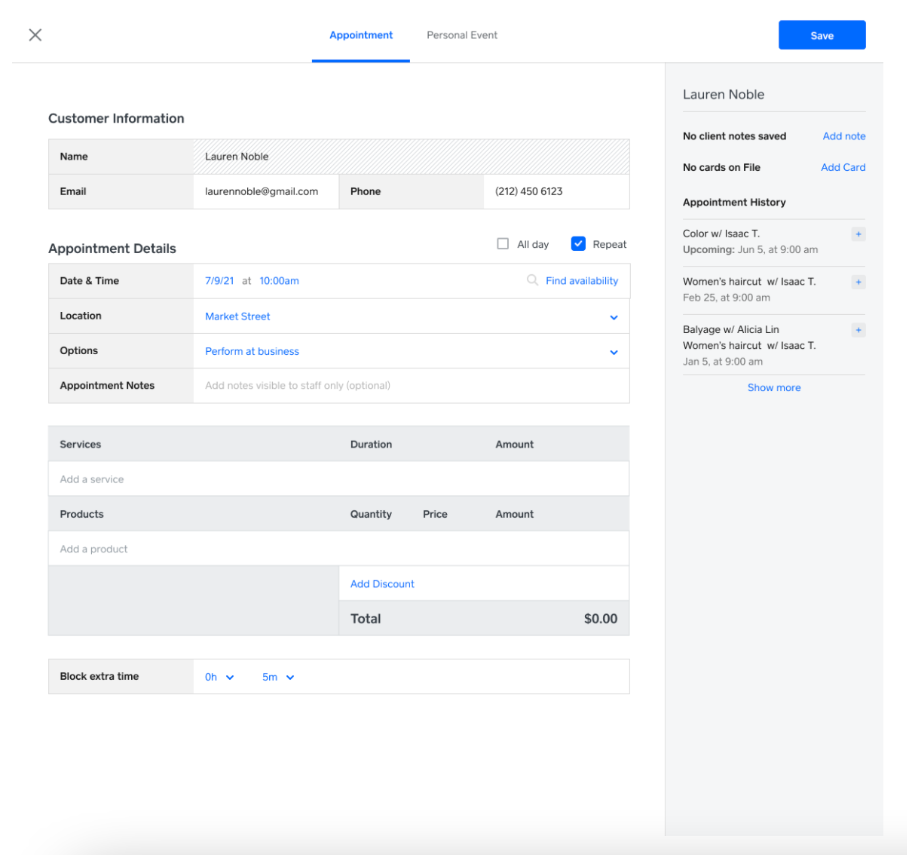
\includegraphics[width=\textwidth]{images/examples/appointment_creating_square.png}
    \caption{Appointment creation interface (Square)}
    \href{https://squareup.com/help/us/en}{Source: Square — Help}
    \label{fig:appointment-creation}
\end{figure}

The appointment creating from Square POS (\ref{fig:appointment-creation}) shows
customer information input table on the top, appointment details in the middle
and services at the bottom (there are also some extra features that we are not
interested in). It offers these important features for employees:

\begin{itemize}
    \item It allows for employees to see all the important information in one page, meaning that there is no need to have several pages open at once.
\end{itemize}

The only thing missing here is choosing the employee that the customer wants to be serviced by, but as the UI is structured in tables and rows clearly, it would be quite easy to add one more row below services for the employee to specify what employee the customer wants to be serviced by. 

We did not find any written user needs in this document that it satisfies.

It satisfies these \textbf{usability objectives:}
\begin{itemize}
    \item \hyperref[OBJ-03]{OBJ-03} The clear UI with seperated tables for customer information, appointment details, services makes employee jobs more quicker and easier. As a result employee satisfaction rises.
\end{itemize}



\begin{figure}[H]
    \centering
    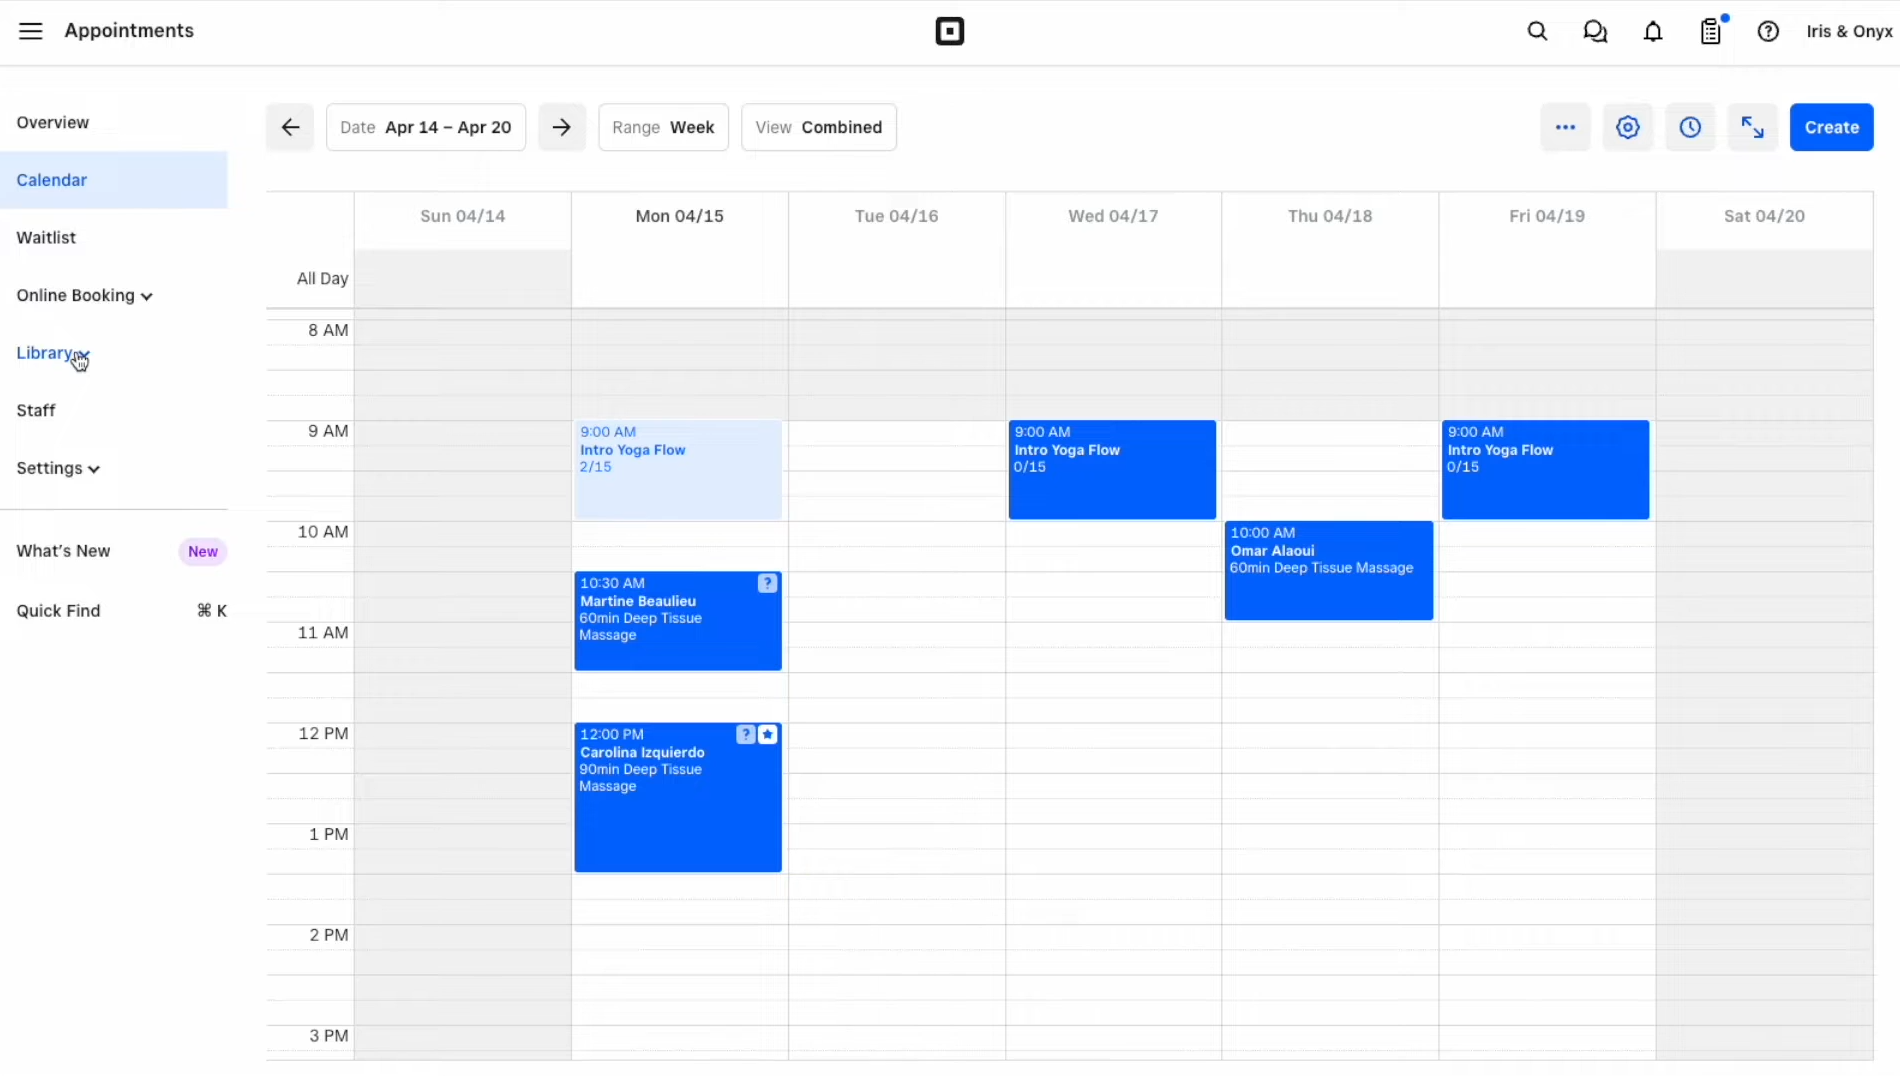
\includegraphics[width=\textwidth]{images/examples/appointments_square.png}
    \caption{Appointments list (Square)}
    \href{https://squareup.com/help/us/en}{Source: Square — Help}
    \label{fig:appointment-list}
\end{figure}

The appointment viewing from Square POS (\ref{fig:appointment-list}) shows a
side bar on the left and a table of appointments on the right. There are also
some filtering options on the top and a search icon (not very visible) on the
top right. It offers these important features for employees:

\begin{itemize}
    \item It allows for employees to quickly see what appointments are coming up and find appointments that need to be changed or canceled.
\end{itemize}

This user interface satisfies these \textbf{user needs:}

\begin{itemize}
    \item \hyperref[UN-02]{UN-02} - It allows for the employee to see which slots are booked and which free.
    \item \hyperref[UN-04]{UN-04} - While not very clear at first as the search icon at the top of the image is quite small, employee can use it to search the bookings.
\end{itemize}

It satisfies these \textbf{usability objectives:}

\begin{itemize}
    \item \hyperref[OBJ-02]{OBJ-02} The system forbids double booking, meaning that the only errors the employee can make are errors like imputing customer name or phone number wrongly.
    \item \hyperref[OBJ-03]{OBJ-03} The employee satisfaction increases as system prevents double bookings and furthermore the booking information in provided clearly in a slot based manner.
\end{itemize}


\begin{figure}[H]
    \centering
    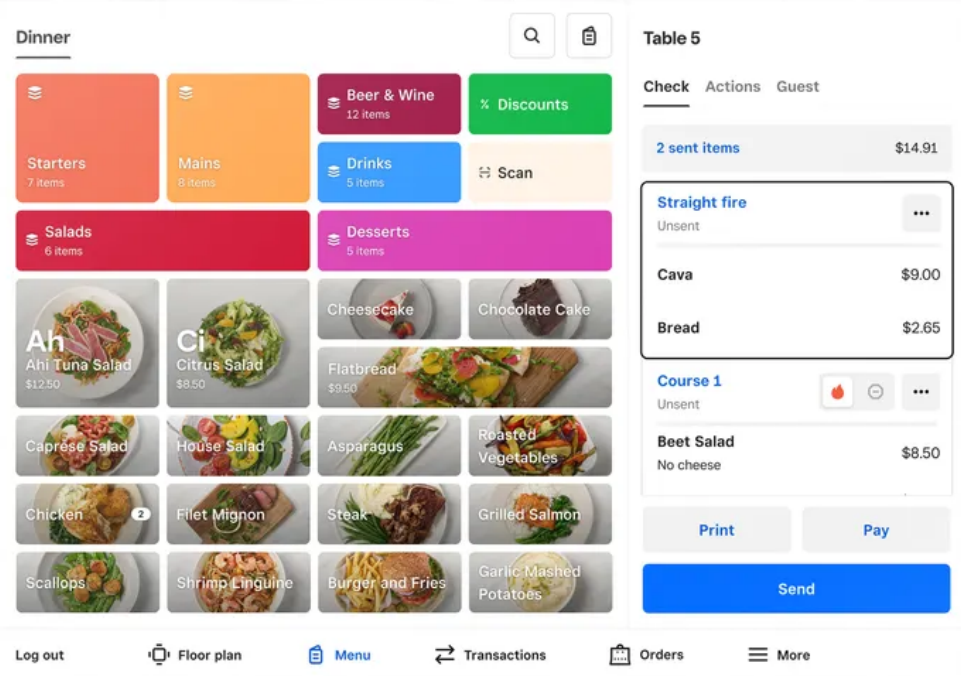
\includegraphics[width=\textwidth]{images/examples/square_orders.png}
    \caption{Orders (Square)}
    \href{https://squareup.com/help/us/en}{Source: Square — Help}
    \label{fig:square-orders}
\end{figure}

The order menu from Square POS (\ref{fig:square-orders}) shows menu information
in table like format on lefts side and the order details on the right side. It
also offers quick navigation buttons on the bottom for floor plan, menu,
transactions, orders and more. It offers these important features for employees:

\begin{itemize}
    \item It allows for employees to quickly choose what the customer from menu wants.
    \item It shows the check simultaneously while new items are added so employee can inform the user what the discounts are available
\end{itemize}

This user interface satisfies these \textbf{user needs:}

\begin{itemize}
    \item \hyperref[UN-01]{UN-01} - It allows for the employee to easily see what orders were added.
    \item \hyperref[UN-06]{UN-06} - The system calculates the total for the employee and also provides a detailed check so the employee does not need to do all that in their head or with a calculator.
\end{itemize}

It satisfies these \textbf{usability objectives:}

\begin{itemize}
    \item \hyperref[OBJ-03]{OBJ-03} The UI allows the employee to simultaneously view menu and order details, reducing mental overhead and the need to memorize in turn increasing employee satisfaction.
\end{itemize}



\begin{figure}[H]
    \centering
    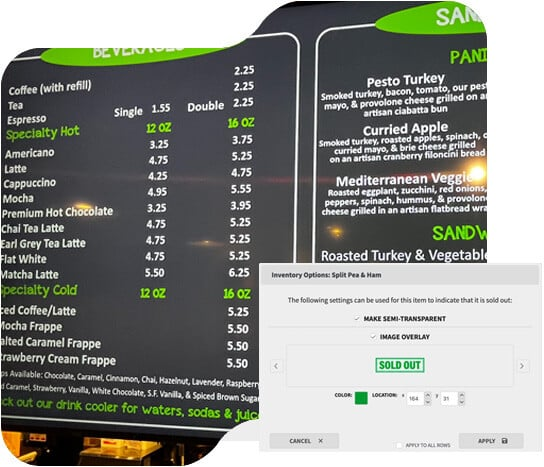
\includegraphics[width=0.7\textwidth]{images/examples/live-menu-square-smartersign.jpg}
    \caption{Live menu (Square + SmarterSign)}
    \href{https://smartersign.com/square}{Source: SmarterSign}
    \label{fig:square-menu}
\end{figure}

The live menu addon for Square POS (\ref{fig:square-menu}) shows information in
a table manner, each item is grouped by category and each item has its price
shown. It also shows some explanation about meals on the right side. It
offers these important features for customers:

\begin{itemize}
    \item It allows for customers to quickly check what is the price of the item they want, if it is available, and in what quantity it is served.
\end{itemize}

It does not show how long it will take to prepare these items but this information could easily be added.

This user interface satisfies these \textbf{user needs:}

\begin{itemize}
    \item \hyperref[UN-09]{UN-09} - The menu allows the customer to seethe availability and preparation time of the meal they want.
    \item \hyperref[UN-10]{UN-10} - The menu clearly shows to the customer which meals are currently available.
\end{itemize}

It satisfies these \textbf{usability objectives:}

\begin{itemize}
    \item \hyperref[OBJ-04]{OBJ-04} - The customers can quickly learn what is in stock so they do not need to ask employee or wait in line.
    \item \hyperref[OBJ-05]{OBJ-05} - The customers will be satisfied as they will be able to quickly make decisions.
    \item \hyperref[OBJ-06]{OBJ-06} - The customers will be able to quickly see how long their meal will take to make.
\end{itemize}

\begin{figure}[H]
    \centering
    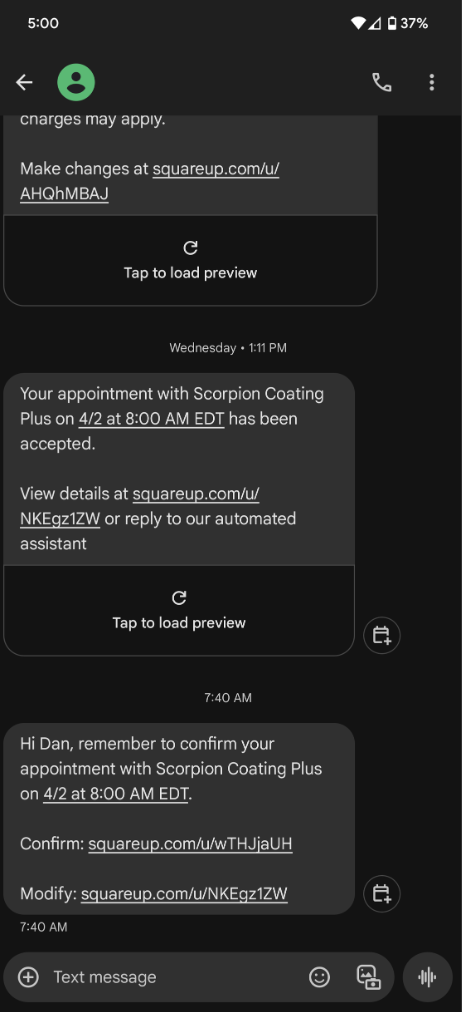
\includegraphics[width=0.5\textwidth]{images/examples/square_SMS.png}
    \caption{Square SMS messages}
    \href{https://squareup.com/help/us/en}{Source: Square — Help}
    \label{fig:square-sms}
\end{figure}

The SMS messages from Square POS (\ref{fig:square-sms}) while not being part of actual UI elements, still showcases that the text has to be clearly structured for the customer to quickly understand the purpose of the message. It offers to customer this information:

\begin{itemize}
    \item It asures the customer that their appointment was confirmed.
    \item It provides the time and the service name.
\end{itemize}


This SMS message satisfies these \textbf{user needs:}

\begin{itemize}
    \item \hyperref[UN-08]{UN-08} - Customers can clearly see when if their appointment status.
\end{itemize}

It satisfies these \textbf{usability objectives:}

\begin{itemize}
    \item \hyperref[OBJ-05]{OBJ-05} - We can expect that customer satisfaction will increase as they will feel well informed by the SMS messages. 
\end{itemize}


% MANAGER STUFF BELOW
% MANAGER STUFF BELOW
% MANAGER STUFF BELOW
% MANAGER STUFF BELOW
% MANAGER STUFF BELOW

\begin{figure}[H]
    \centering
    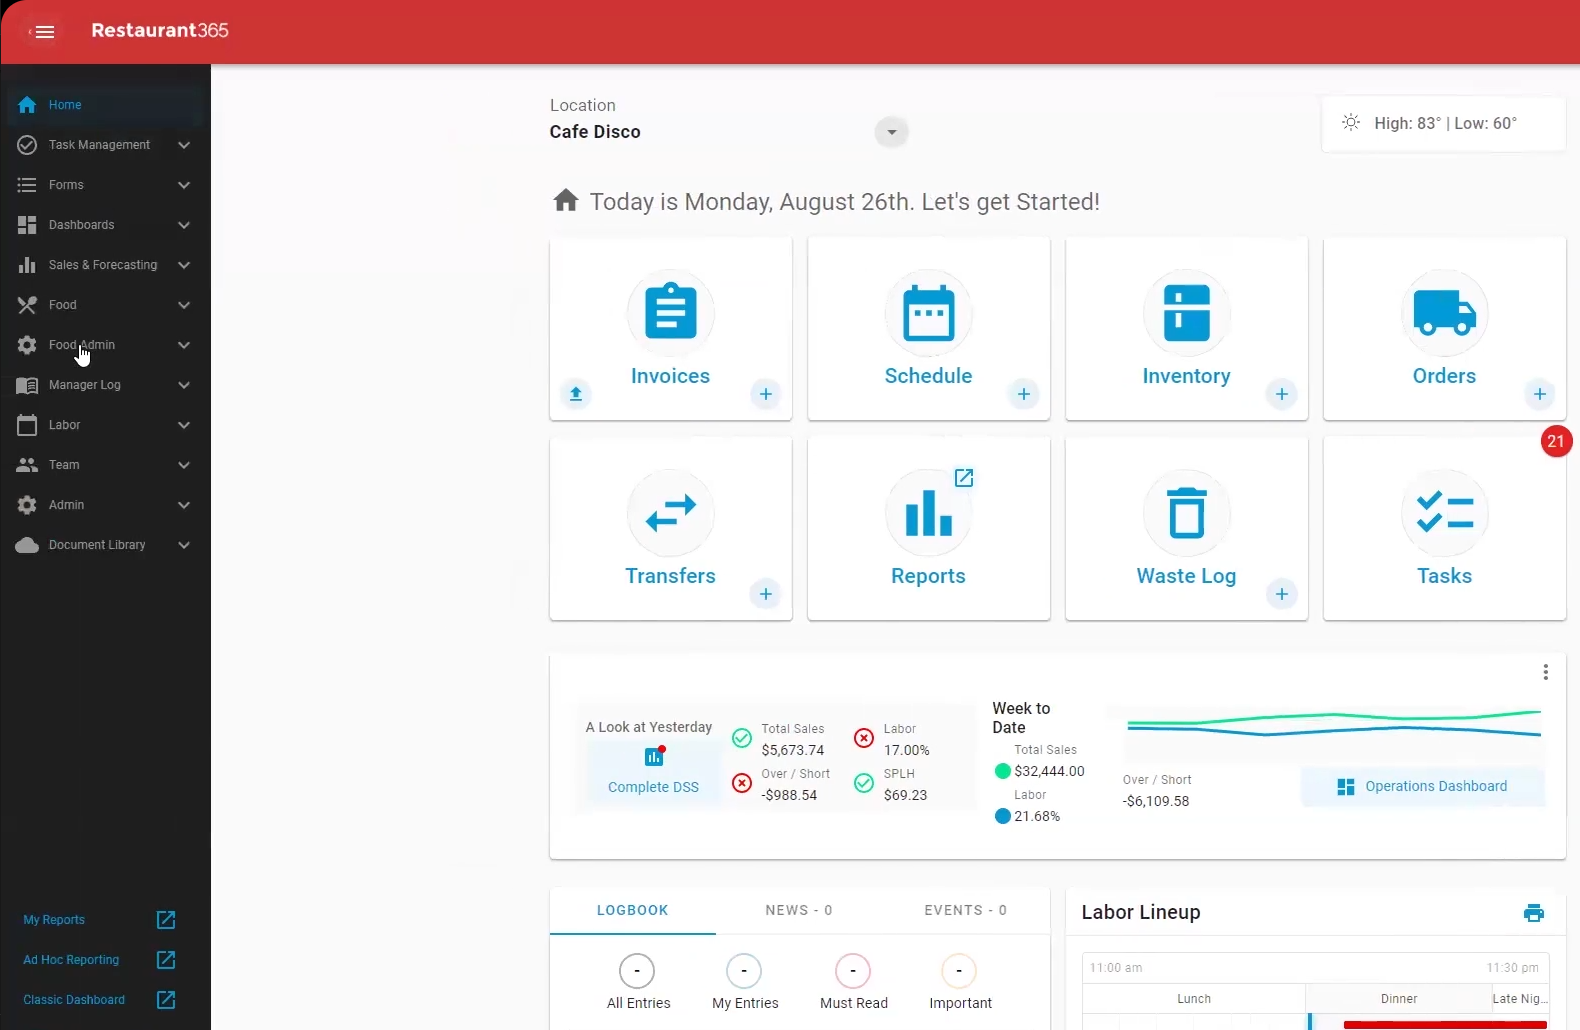
\includegraphics[width=\textwidth]{images/examples/homepage_r365.png}
    \caption{Homepage dashboard (Restaurant365)}
    \href{https://www.restaurant365.com/resource-category/videos/}{Source: Restaurant365 — Videos}
    \label{fig:homapage-dashboard}
\end{figure}


The homepage from Restaurant365 (\ref{fig:homapage-dashboard}) has a very clear
layout by having the side bar on the left and the main content on the right. It
also shows all the most important information and navigation buttons on the
right side. It offers these important features for business owners: 

\begin{itemize}
    \item there is quick access to transfers, reports, logs, tasks, invoices and other features.
    \item The graph below allows for quickly viewing what are the business profits currently and allows for managers to understand if any action is needed and if any anomalies appear.
\end{itemize}

These these \textbf{user needs are satisfied:}
\begin{itemize}
    \item \hyperref[UN-14]{UN-14} - business owners can clearly see in this UI what are the profits by the business. In addition, they can quickly navigate to the reports section by just clicking the Reports button in homepage.
    \item \hyperref[UN-15]{UN-15} - business owners can quickly click navigate to the inventory section by just clicking the Inventory button. There they will be able to do all the necessary actions with inventory management.
\end{itemize}

It satisfies these \textbf{usability objectives:}

\begin{itemize}
    \item \hyperref[OBJ-07]{OBJ-07} - business owners can clearly see and access the most important information like inventory management, invoices, reports, etc. in just one click from the homepage.
    \item \hyperref[OBJ-08]{OBJ-08} - business owners do not need to memorize the user interface a lot as all the most important features are clearly displayed in big icons and buttons and are quickly accessible through the homepage. Furthermore the homepage also contains a graph for quickly looking up the business profits and also clicking the operations dashboard button for more information so business owners do not need to search it and remember where the profit information is displayed.
\end{itemize}






\begin{figure}[H]
    \centering
    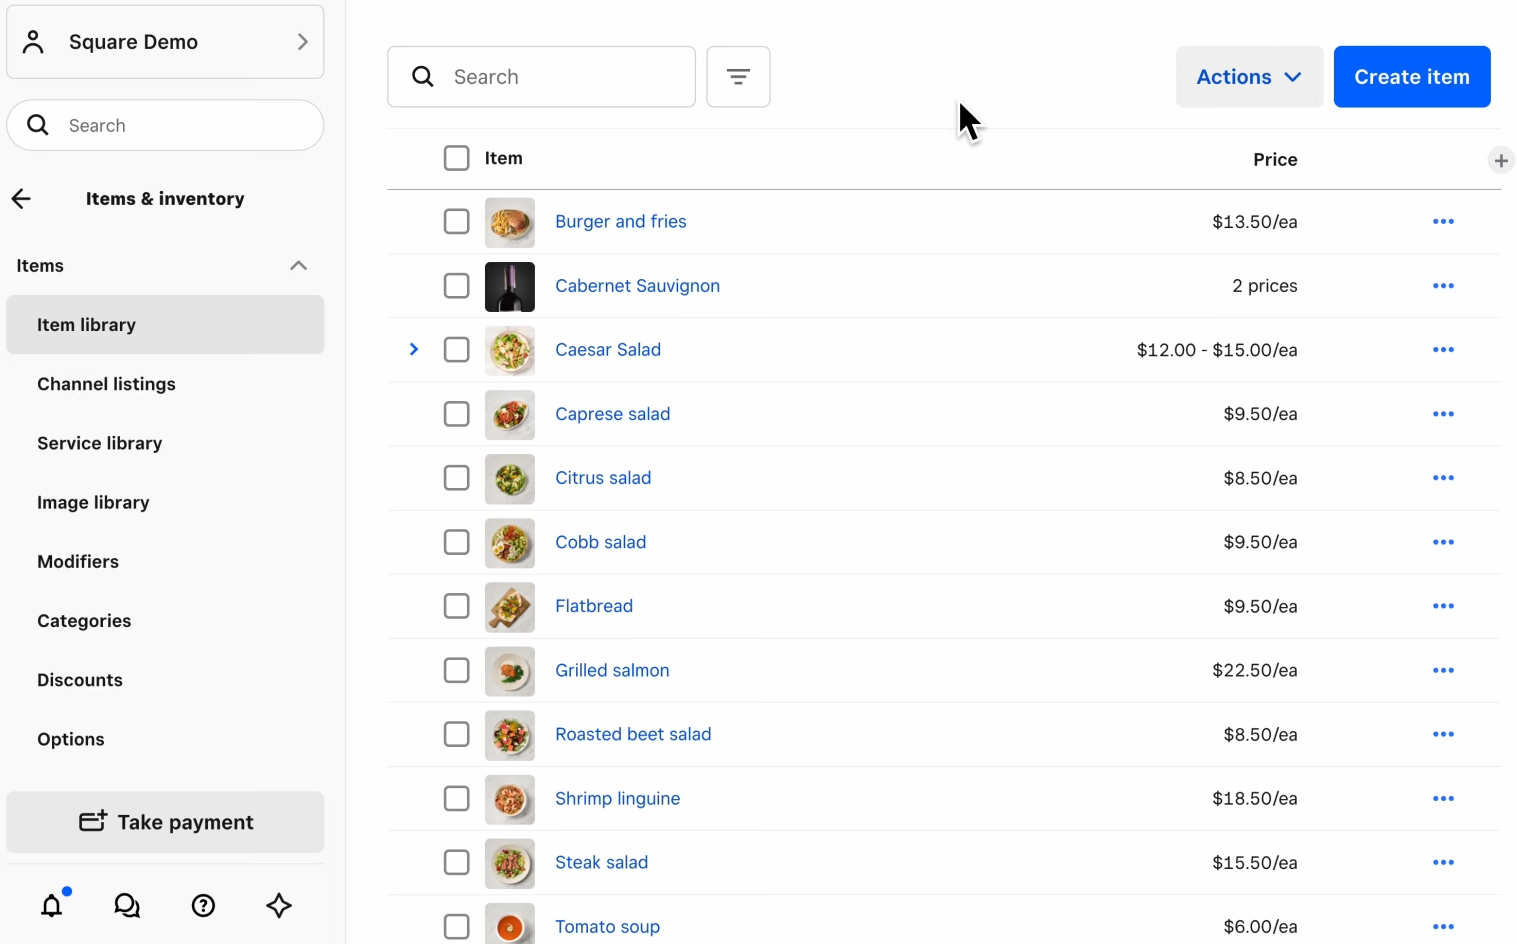
\includegraphics[width=\textwidth]{images/examples/item_menu_square.png}
    \caption{Menu item configuration (Square)}
    \href{https://squareup.com/help/us/en}{Source: Square — Help}
    \label{fig:menu-item}
\end{figure}

The item management from Square POS (\ref{fig:menu-item}) has a clean layout by having the side bar on the left and the main content on the right. Each item has
a clear image for quick recognition and each item can be clicked to see more details. It
offers these important features for business owners: 

\begin{itemize}
    \item Managers can change the prices, discounts of items, add new items and their modifiers as seen in the side bar.
\end{itemize}

We did not find any used needs in this document that this user interface would satisfy.

It satisfies these \textbf{usability objectives:}

\begin{itemize}
    \item \hyperref[OBJ-08]{OBJ-08} The business owners are ale to quickly navigate the inventory and the rest of inventory options in side bar.
\end{itemize}

% \begin{figure}[H]
%     \centering
%     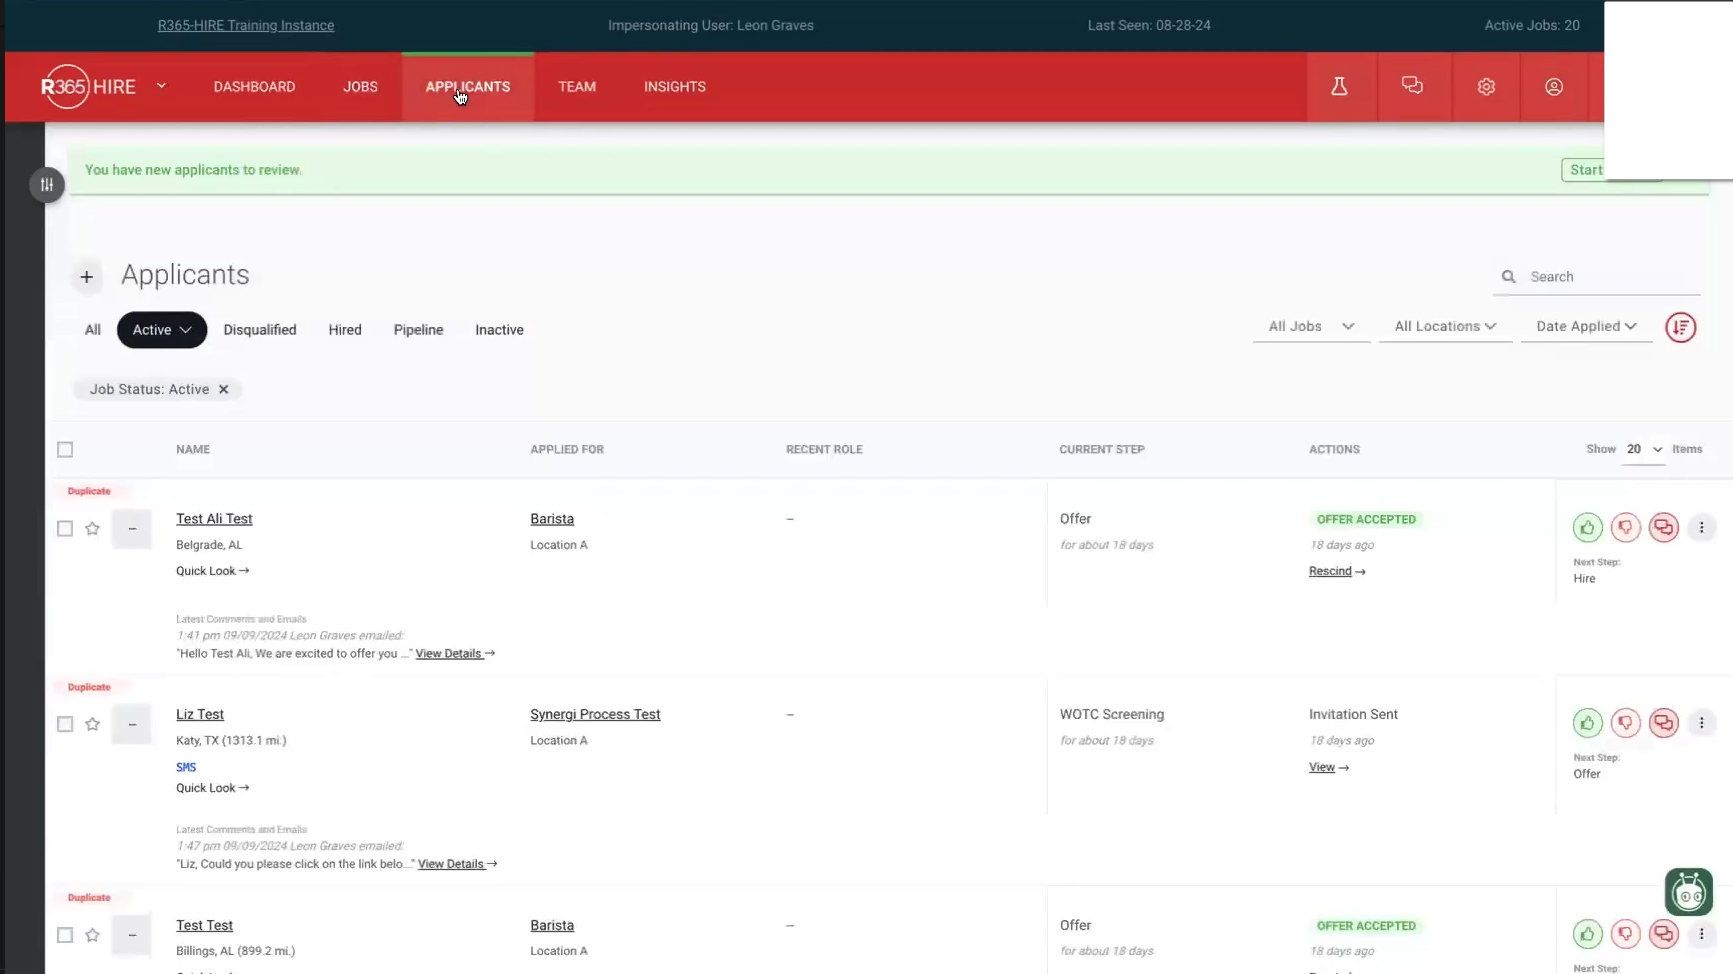
\includegraphics[width=\textwidth]{images/examples/applicants_r365.png}
%     \caption{Applicants management interface (Restaurant365)}
%     \href{https://www.restaurant365.com/resource-category/videos/}{Source: Restaurant365 — Videos}
%     \label{fig:applicants-management}
% \end{figure}

% The applicants managements from Restaurant365 (\ref{fig:applicants-management}) interface offers these important features for business owners:

% \begin{itemize}
%     \item It allows for business owners to quickly hire new people, decide who will be fit for the job and who will not be.
% \end{itemize}

% This user interface satisfies these \textbf{user needs:}

% It satisfies these \textbf{usability objectives:}




% \begin{figure}[H]
%     \centering
%     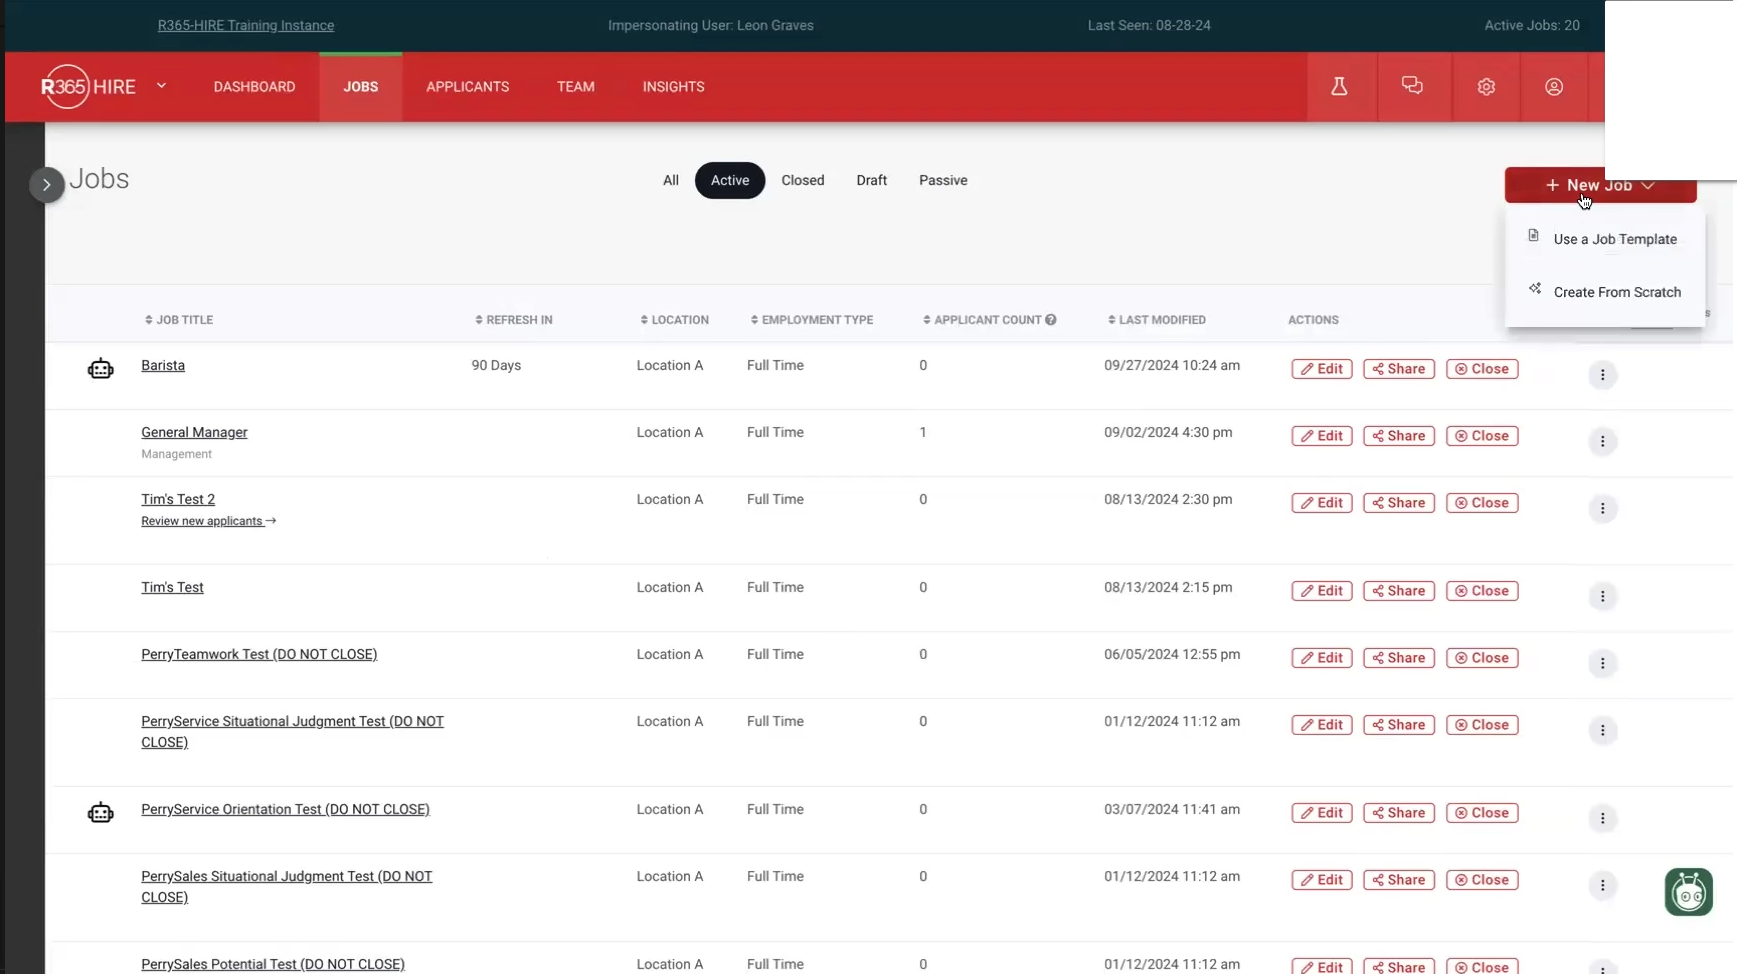
\includegraphics[width=\textwidth]{images/examples/jobs_r365.png}
%     \caption{Jobs overview (Restaurant365)}
%     \href{https://www.restaurant365.com/resource-category/videos/}{Source: Restaurant365 — Videos}
%     \label{fig:job-overview}
% \end{figure}

% The job overview interface from Restaurant365 (\ref{fig:job-overview}) offers these important features for business owners:

% \begin{itemize}
%     \item It allows quickly for business owners to see what job titles their business has and how many employees specify in that title.
%     \item It allows for quick creating, editing and closing of these jobs.
% \end{itemize}

% This user interface satisfies these \textbf{user needs:}



% It satisfies these \textbf{usability objectives:}

\begin{figure}[H]
    \centering
    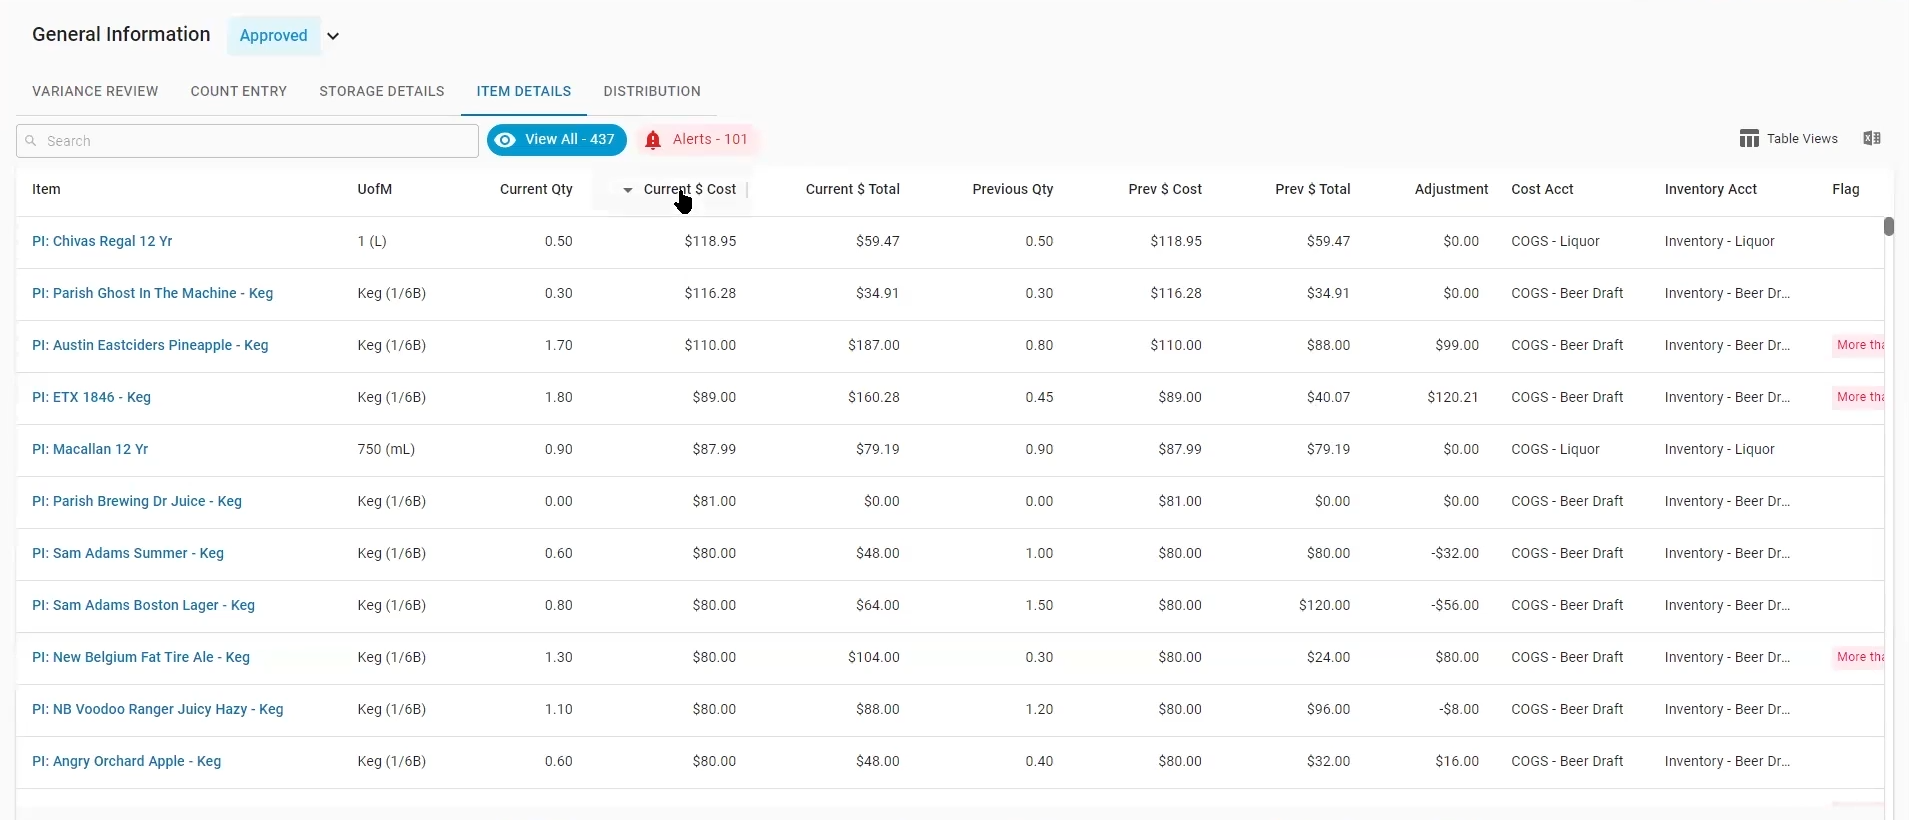
\includegraphics[width=\textwidth]{images/examples/inventory_r365.png}
    \caption{Jobs overview (Restaurant365)}
    \href{https://www.restaurant365.com/resource-category/videos/}{Source: Restaurant365 — Videos}
    \label{fig:inventory-overview}
\end{figure}

The inventory overview interface from Restaurant365 (\ref{fig:inventory-overview}) displays information in a simple table format and
offers these important features for business owners:

\begin{itemize}
    \item It allows quickly for business owners to see what items are available in inventory, their quantity, price changes.
    \item It allows for business owners to see flags associated with items, for example if the item is below par level.
\end{itemize}

This user interface satisfies these \textbf{user needs:}

\begin{itemize}
    \item \hyperref[UN-15]{UN-15} The business owners can optimize their supply orders based on the inventory information.
\end{itemize}

It satisfies these \textbf{usability objectives:}

\begin{itemize}
    \item \hyperref[OBJ-09]{OBJ-09} The business owner satisfaction will rise as they will be able to have quick access to clear tables for inventory data and analyze it more efficiently.
\end{itemize}



\begin{figure}[H]
    \centering
    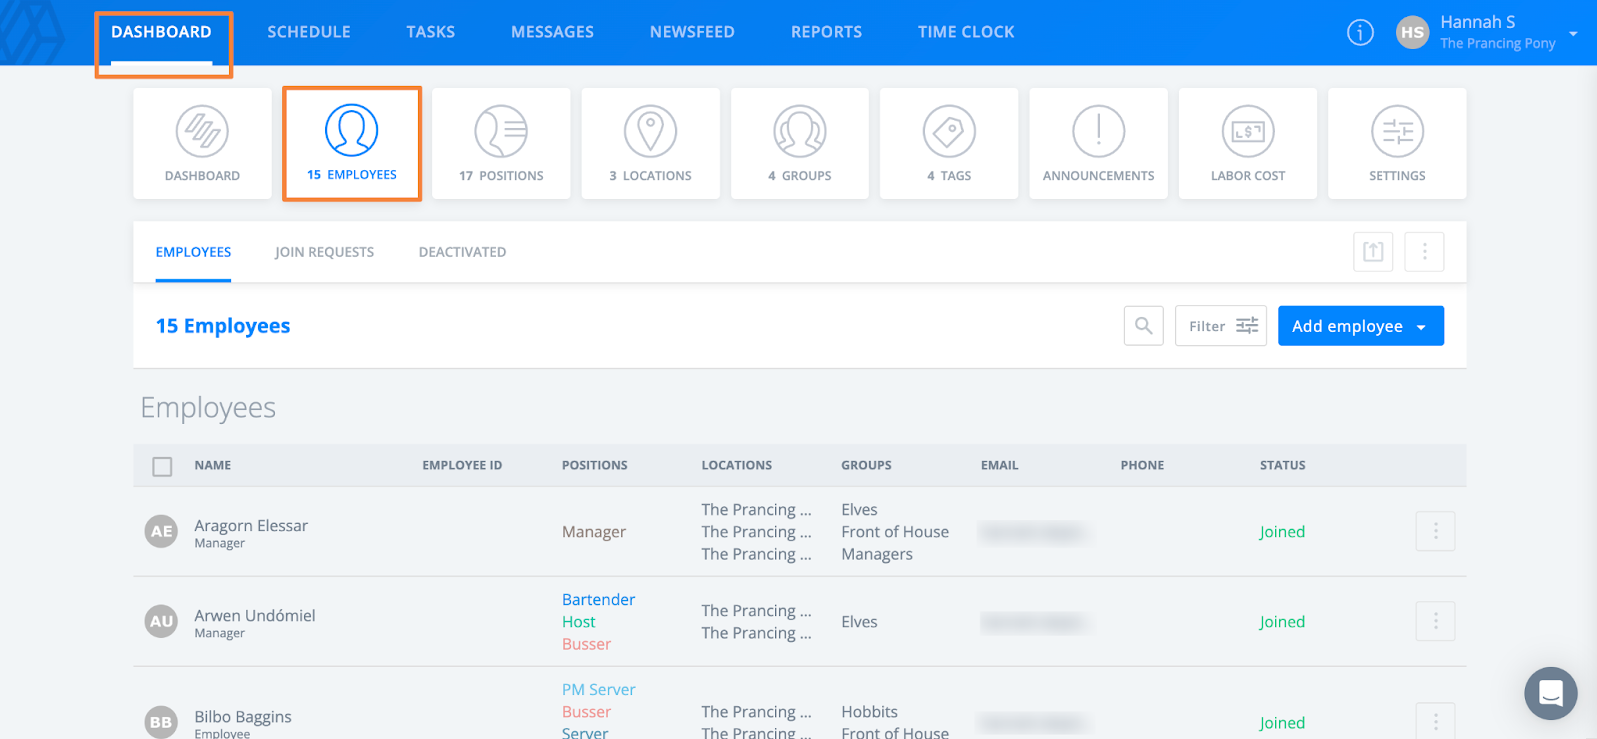
\includegraphics[width=\textwidth]{docs/computer-interaction/1 assignment/images/examples/toast+Sling_employee_management.png}
    \caption{Employee overview (Toast + Sling)}
    \href{https://support.getsling.com/en/articles/8981593-sling-toast-admin-manual}{Source: Sling documentation}
    \label{fig:employee-overview}
\end{figure}

The employee overview interface from Toast with Sling add-on
(\ref{fig:employee-overview}) has quite nice layout, the top row has most used
functionality buttons and the rest of the page is filled on information based on
what button is clicked. It offers these important features for business owners:

\begin{itemize}
    \item It allows quickly for business owners to see what employees they have hired and what their roles are.
    \item It allows for quickly editing employee roles, payout, etc.
\end{itemize}

This user interface satisfies these \textbf{user needs:}

\begin{itemize}
    \item \hyperref[UN-13]{UN-13} - While the dashboard does not explicitly state how the employees perform well, it does allow to see data like positions, groups. Furthermore there is also tasks button in the app bar which we can assume would allow to see for the business manager how quickly certain tasks by certain employees are performed.
\end{itemize}

It satisfies these \textbf{usability objectives:}

\begin{itemize}
    \item \hyperref[OBJ-08]{OBJ-08} - Business owners can quickly navigate the dashboard, all the important features are displayed in the app bar. In short, the UI does not require extensive memorization and most features are reached in one click.
\end{itemize}








% sestadieni reikes ikelti.

% didinti verslinguma nera poreikis, nebus tokio mygtuko

% tarpininkas turi gauti kazkokius notifications
% poreikiai bus padavejo GUI.

% tam tikros funkcijos ateis is pasakotojo pasakojimo, atsekamumo matrica
% customer nera usability objectives, nes jis naudoja per tarpininka, sita
% reikia pamineti.

% ook for existing design examples that could inspire future design solutions
% (at least 5). - geri is kitu sistemu, screenshot, kuriai funckijai cia galetu
% tikti, kodel manom kad otks dizainas tiktu.


% paziureti kaip needs rasomi pagal standarta, skaidrese, angliskai ir
% lietuviskai kazkur parasytas paaiskinimas

% atsekamumo matrica -  viena galima vienam dalykui, kita kitam. atsekamumas
% turi parodyti kad poreikis is kazkur isplaukia, is kurio scenarijaus, is kurio
% pasakojimo, is kurio user story.

% jeigu rasome kaip sekmes kriteriju kad turi vartotojas gauti kazka per viena
% min tai reiskia kazkur parasyta kad adabar jis ta gauna ilgiau nei viena min.


% tekste paveiksliuka pacituoti, pasakyti kodel jis yra ten, koks poreikis.

% ------------------------

% primari ir secondary stakeholder kursime sasaja
% poreikis - ka veiks vartotojas ir ka gaus ekrane




% ------------------------



% ------------------------
% PACT stuff below
% ------------------------



% reikia sistemizuoti kokioje situacijoje ko reikia, labiau detaliau issiaiskinti stakeholder needs.
% reikia atlikti naudojimo konteksto analize, kaip tos funkcijos isilies i vartotojo esama gyvenima. Mes galvojame apie naudojima ir konteksta vis dar.
% Naudojimo kontekstas - kaip veiklos itakoja technologiju kaita ir technologiju kaita veiklas, po to kalbesime apie pagrindines zmoniu charakteristikas, kas, kokiose veiklose ir problemas kurias norime spresti, kokiame zingsnyje kas ten stringa, kokioje aplinkoje ten vyksta, kokios tech naudojamos ir ka galime pasiulyti.
% Naudojimo kontekstas - kombinacija vartotoju, uzduociu, resursu, tikslu. Fizines, socialines, technines, kulturines, organizicines aplinkos. Jas riekes issaiskinti ir aprasyti kaip dabar veikia tas vartotojas, ka tie pasakojimai turi atspindeti: turi buti aiskus visi aspektai, kas, kokie tisklai, aplinkos, kokiais prietaisais, programomis naudojasi ir t.t.
% PS inzinerijos standartas - naudojimo kontekstas pagrindinis informacijos reikalavimu saltinis.
% Vystimasis yra begalinis ciklas, yra zmones betkokio amziaus, kutluros, jie veikia kazkokiam kontekste (requirements), tame kontekste kyla nauji reikalavimai naujoms technologijosm, naujos technologijos sudaro galimybe keistis veiklos, vel atsiras nauji reikalavimai ir t.t. gaunasi begalinis ratas.
% naujos interaktyvios tech - prisidedame dabartines zinias, sukaupta patirti ir kuriame naujus reikalavimus. Suvokdami kazkokius nepatogumus, koks yra stovis, kokias galimybes mes galime isnaudoti su technologijomis mes pasiulome sprendimus, naujas veiklas.

% People, context, activities, technologies

% ____________________________

% People - kokiomis salygomis veikia, ju fizines galimybes, darbo vieta, veikimo
% aplinka kur bus naudojama technologija, zmoniu ugis, aukstis, antropronetiniai
% dalykai? ivestis isvestis, klaviaturos ir t.t. Nera vidutinio vartotojo,
% universali technologija reiskia kad visiem patogu naudotis, zinoma yra tam
% tikri kompromisai, reikalavimai turi tilpti i budget. Pvz.: ekrano padetis,
% ryskumas, kontrastas, color blindness, motion sensitivity, hearing etc. etc.
% Musu varottoju tarpe jeigu yra vyresni zmones tai turime i tai atsizvelgti,
% mygtukai didesni ir t.t. Kokia turi buti darbo aplinka kad zmogus nepavargtu,
% nebutu broko, darbo vieta turi buti tokia kuri leistu islaikyti darbinguma.

% psihologinis erdviu suvokimas, kai kurie pasiklysta, kai kurie gerai
% orientuojasi erdvese. kalbos skirtumai, kai kam gali buti izeidzianti kalba,
% kai kam ne...

% isiminimas, trumpalaikis isiminimas, sprendimu priemimas, komunikacija,
% paieska - mes turime sias veiklas kurioms kuriame technologijas.

% socialiniai skirtumai - itakoja motyva pirkti nauja technologija, gali
% atsirasti stiprus motyvas, pvz bendrauti nuotoliniu budu, todel zmones ismoks
% tai. skirstosi tipai, begginer, inermediate, expert zmoniu. pvz bileteliu
% popieriniu nenupirksi, tai beggineriai turi tai naudoti... vidutiniskai patyre
% kai reikia tia naudoja o taip tai nenaudoja. profesionalai - kiekviena diena
% naudoja. beggineriu ir expertu poreikia yra labai skirtingi.

% kad pradedantysis galetu naudotis technologija tai ji turi vesti uz rankos,
% pvz vedlys, jis vedamas uz rankos.

% ekspertai - jiem reikia greicio, juos vedlys erzins.

% vidutiniskai patyre - reikia prisiminti greitai.

% jie visi turi skirtingus poreikius, reikia suprasti su kuo turime reikala.


% Mental model - mintinis modelis, koki vaizda suformavo vartotojas savo
% galvoje, mes bandome tai sufprasti, tai suvokimas kas ir kaip gali naudoti
% technologijas. Mintinis modelis nepilnas, nestabilus, mes negalime visko
% prisiminti, kazkas isilaiko ilgalaikeje atmintyje, kazkas dingsta.
% Analizuojame o ka dabar naudoja vartotojai, analizuojame ju mintines zinias.
% Mintinis modelis kuriamas saveikaujant su sistemomis, su kokiomis sistemomis
% saveikauja toki ir turesime mintini modeli.

% Nustatymas vartotojo igudzius yra musu tikslas. kokio amziaus, lytis, fizines,
% issilavinimas, kulturinis, motivacines galimybes, tikslai, asmenybe.
% Projektavimo tikslai turi susieti su tais skillais. musu tikslas kad
% vartotojai pilnai isnaudotu ka suprojektavome, norime kad is begginer greitai
% pereitu i intermediate.

% Pavyzdiziui kai pirma karta paleidziame programa, gali issokti gidas, padeti
% beginneriams, o kam nereikia tai gali uzdaryti, uzdaro vidutiniskai patyre.
% Ekspertam reikia kuo greiciau dirbti, kas stabdo (rankos kelimas nuo peles iki
% klaviaturos, galime sakyti kad viska darytu ant klaviaturos).

% kiek tu sluoksniu design reikia? tai papildomos islaidos ir t.t.


% begineriam programa turi pasakyti ka ji gali daryti, pagrindiniai dalykai ka
% ji daro, begineriu nera daug bet jie yra ir pirmi naudotojai todel jiems
% reikia viska paaiskinti. po keliu kartu dauguma begineriu tampa intermediate.
% intermediate svarbu matyti, isnaudoti visas funkcijas kurias jie zino kad yra,
% gebeti viska surasti, pazengusias funkcijas. GUI visas pagrindines ir
% pazengusias funkcijas rodo ir galima greitai surasti Ekspertu nera daug,
% kazkam galbut greiciau reikia.

% kuri viekla daznesne, ta turi buti arciau ekrano.


% Universal usability - prieinamas visiems, ir neigaliems. Panaudojamumas +
% prieinamumas = universalumas. kas aktualu, kam kuriame sistema, i sita turime
% atsakyti.



% Reikia pamineti demographics, age, occupation, gender (jei reikia),
% disabilities. Motyvacija ismokti technologijas, jomis naudotis. Naudojamos
% technologijos ir prietaisai, IT lygmuo, skillai.

% ____________________________

% Veiklos - reikia ne specifines mineti, o laiko aspektu daznas ar retas,
% bendradariavimo aspektus, individualus ar organizaciniai, tos veiklos
% sudetingumas, pasekmes, ar kritines, kokio tipo turinys toje veikloje.

% Daznis jos pirma charakteristika, jos trukme antra, laiko spaudimas, ar veikia
% ramybes busenoje ar skubos. Ar tai viena atomine veikla ar zingsniai yra, ar
% testine is zingsniu tai kazkuriame zingsnyje vartotojas gali sustoti. atsako
% laikas. Bendradarbiavimas, vienas ar grupeje, kaip zino kas ka padare, kaip
% koordinuoja, komunikuoja. Sudetingumas veiklos, ar veikla apibrezta ar ne,
% reikia suteikti vartotojui galimybe narsyti ivairias veiklas, kur vartotojas
% nori narsyti, kaip vartotojas supras ar nutrauke zingsni ir t.t. tai
% sudetingumas. kaip supras kad klaida padare, ar tai aktualu. kokie duomenys
% vaiksto, kiek ivesti ten reikia, kokia ten isvestis dabar ir kas siuloma, turi
% buti realiu laiku atnaujinamas turinys, kad nebutu blogai pavaizduotas, blogai
% atnaujintas.

% Ne pacios veiklos idomios bet ju charakteristikos.

% ____________________________

% Aplinka - fizine, kur vyksta ta veikla, patalpoje, uz patalpos, jeigu fizine
% aplinka lauke, tai skirtinga temperatura, kaip vartotojas su pirstinemis ar
% per lietu gali naudotis, apsvietimas, triuksmas ir t.t.

% Socialine aplinka - individuali, o gal grupine, ar privatumas aktualus, ar
% visi vienodu teisiu, ar yra super adminas.

%  Organizacinis kontekstas - teises ir t.t.

% ____________________________

% Technologijos - ka dabar naudoja zmones, kokias technologijas, ka jie dabar naudoja, tia itakoja ju mintini modeli, kaip jie dabar iveda informacija?

% Kokias technologijas naudosime - kompiuteris, programele telefone, ar t.t.

% Turime susivokti kokiu techniniu ir sistemu reikia. Kas yra geras turinys ir kokios charakteristikos galetu tobulinti tai, balsu ivedimas, AI ar whatever.

% kokia informacija ir funkcijos reikalingos sistemai, kas tures buti zinoma norinciam naudotis sitema.


% Interaktyvus produktas turi atitikti tai ko nori zmones, jis negali sugriauti kontekto, jis turi tai pagerinti.

% musu uzdavinys visus siuos dalykus issiaiskinti, parasyti kiekvienai pirminei ir antrinei vartotoju grupei aprasyti siuos dalykus ir po to dar kitai savaitei galime pradeti rasyti poreikius kas isto isplaukia ir kokiu funckiju riekia

% \sectionnonum{Results and conclusions}
% For details of what needs to be written in this section, please refer to the methodology requirements of the respective programme.


% ------------------------
% User Studies
% ------------------------

% Suvokimo procesas - nelabai gali issivaizduoti, projekte vyksta kuryba.
% Jeigu viskas patogu tai niekas nepastebi, jeigu kazkas nepatogu tai visi pastebi..

% Yra PACT sistema kuri apibendrina viska. Patys bendriausi reikalavimai yra
% vartotoju poreikiai, tai nevisai kaip reikalavimai. Poreikiai - ka vartotojas
% nuveiks, ka matys sistemoje.

% Vartotojau nori kad processas butu sklandus, intuityvus <- negeras aprasymas,
% ar cia bus mygtukas ar kazkas ekrane, cia yra labiau verslo lukesciai.



% Scenarijai turetu pateikti zingsnius kaip vartotojai dabar veikia, 
% what
% how
% any problems /\<- visa sita jau padarem

% ------------------------
% Koki tyrima darom
% yra kokybiniai ir kiekybiniai tyrimai
% kiekybiniai - apklausos, anketos, statistika, daug zmoniu, galime apibendrinti visai populiacijai, bet gauname mazai izvalgu
% kokybiniai - interviu, stebejimas, mazai zmoniu, gauname daug izvalgu, bet galime atsidurti klaidingoje situacijoje, negalime apibendrinti visai populiacijai


% kiekybiniams reikia didelio biudzeto.

% kiekybiniame tyrime suzinome nuostatas, problemas su laiku pradeda kartotis info.


% human centered design - suzinome prie ko zmones priprate ir atitinkamai
% kuriame technologijas. kokios veiklos daznos, retos, danzesnes veiklos
% pradiniame ekrane, retesnes kitame, etc.


% PERSONAS - isgrynina visas iskalbas kalbant su tam tikra vartotoju grupe.
% persona gaunama pakalbant bent su keliais atstovais is tos vartotoju grupes.
% persona yra konkretus atstovas skirtingu vartotoju grupiu.
% tikslai, prasmingos veiklos isskiriamos.


% zmones kurie daug zino ir kurie nenaudoja mainstream technologijas yra geras
% info saltinis. nereikia kalbeti su mainstream, uzkart galime suzinoti kas
% blogai su tuo mainstream. Gausime gera izvalga, kokie trukumai su ta
% mainstream technologija.



% 1 setting goals - atlikti PACT analize 

% 2 identifikuoti dalyvius, nuspresti is
% ko rinkti info (suinteresuotu analize jau atlikome), probability sampling
% (paimame atsitiktiniu budu zmones) arba non probability sampling (krastutiniu 
% grupiu). Saturation sampling - su visais kalbame kol nebelieka naujos info.

% 3 Relationship with participants - susitarti su vadovybe kad galime kalbinti
% zmones, virsininkas turi pristatyti kad bus toks tyrimas, etc. etc. Informed
% consent - pasiraso kad sutinka dalyvauti.

% 4 Triangulation - vienas info saltinis mazai, turi buti bent keli scenarijai,
% kad zinotume skirtingus poziurius, juos derintume.

% 5 Pilot studies - pabandome su vienu ar keliais zmonemis, kad pamatytume ar
% viskas ok, ar klausimai aiskus, ar suprantami.


% Interviews

% Pirma buna nestrukturizuoti, kuo toliau tuo labiau strukturuoti, tikslinames
% funkcionalumus, pozymius.

% semi strukturuoti - yra pagrindiniai klausimai, bet galima klausti ir papildomai

% group inteviesws - diskusijos, su keliais kalbam.

% vengti ilgu sakiniu, ar, ir, zargonu, vengti stumti i viena ar kita puse.

% fokuso grupe - atstovai is skirtingu grupiu, kai isriskeja skirtingi
% poziuriai. reikia kompromisiniu sprendimu.



\printbibliography[title = {References and sources}]

\end{document}

